\title{HMRS: Hierarchical document management for evidence-traced retrieval}
\author{Author Name\and Co-author Name}

\begin{document}
\maketitle
\begin{center}Affiliation Department, University,
City, Country\end{center}
\begin{center}Correspondence: \href{mailto:author@example.com}{author@example.com}\end{center}

\section*{Abstract}

Retrieval from evolving document collections depends on placement,
descriptions and index consistency. HMRS is a self-hosted system managing
collections, documents and segments through catalogue, shelf, document and
segment views. A November disk inventory found at least one stored part for
each of 100 target papers. A separate rename test exposed nine stale vector
entries, removed by re-indexing.

On a separate ten-domain benchmark of 72 questions, a scripted selector reached
the labelled collection in 72 cases with full route cards and 37 with nominally
name-only cards; this configuration contrast does not isolate description effects.
Combining document and vector chunk windows returned annotated target strings
on 48 questions in the latest seven-arm rerun, compared with 36 for the
baseline. Earlier records gave 52 versus 37 and 51 versus 39 on the same
questions. In the frozen record the combined configuration's trace-recorded
text was about ten times the baseline's and 1.3\% of a mechanical full scan's;
the latest campaign omitted the full scan. These measures do not establish
answer support. In a separate replay of sixteen candidate pools, fusion order
retained 15 top-five hits and verifier-score ordering retained seven. The
results illustrate how collection metadata, reading scope and candidate order
affect evidence access in the evaluated configurations.

\noindent\textbf{Keywords:} Knowledge document management · Document classification · Hierarchical organisation · Tiered retrieval · Evidence verification · Model Context Protocol

\section{1. Introduction}


Enterprise documents preserve regulations, failure analyses and operating
procedures. To answer a question from these materials, a retrieval system
must reach the right collection, identify a document and expose the passage
that supports the answer. Each step depends on earlier management decisions.
A collection description guides the search, a document must be listed on
the selected shelf, and the index must point to its current location.
An accurate passage ranker has little opportunity to recover evidence that
the access path never reaches.

Document acquisition, organisation and retrieval are often evaluated at
different boundaries. Enterprise content management studies document
governance [1, 2], while metadata
quality and tagging determine how users discover those documents
[3, 4]. Distributed
information retrieval addresses the selection of collections
[5, 6]. Retrieval-augmented generation
(RAG) and agentic retrieval add passage ranking and tool-guided evidence
access [7, 8, 9, 10].
HMRS connects these responsibilities. It makes collection membership,
document metadata and source references available from ingestion through
query time, so that an operator can trace a failed search to the stages
that supplied its candidates.

The Hierarchical Management Retrieval System (HMRS) is a self-hosted
knowledge document platform. An ingest agent uses parsed content to select
a collection and describe the document. Management operations update the
files, tree registry and library metadata, and reconciliation checks them
against one another. At query time, a catalogue-first search uses collection
and document descriptions to reach source passages. A pinned search begins
within a selected collection, and an optional server-side evidence gate
returns scored passages with source coordinates. The access policies use the
same managed state, so their choices can be traced independently of parsing
or index maintenance.

\noindent\textbf{Contributions.}
\begin{enumerate}
\item \textbf{A management model for the state behind retrieval.} HMRS
organises knowledge documents as collections, documents and segments, and
connects these managed objects to catalogue, shelf, document and segment
views. Collection membership, descriptions and source references link the
management of documents to the choices made during evidence access
(Section~3).
\item \textbf{A content-informed document lifecycle.} The acquisition
workflow uses parsed content to select a collection and derive document
descriptions and tags. Management operations and reconciliation checks
connect the document files, tree registry and per-library metadata, while
index and retrieval probes help expose stale state after changes
(Sections~4--5).
\item \textbf{Agent access across management levels.} MCP interfaces expose
the catalogue, document descriptions, source documents and indexed passages
to an agent. Catalogue-first and pinned policies let the agent narrow a
search using managed descriptions or start within selected collections
(Section~6).
\item \textbf{A source-traceable evidence gate.} An optional server-side
gate fetches candidate text, scores its passages against the question, and
returns admitted passages with source references and error information.
Candidate ordering is a separate decision made by the calling workflow or
hybrid tool. Answer instructions distinguish a completed search without
support from an incomplete execution
(Sections~6.1 and~6).
\end{enumerate}

\subsection{1.1. Research questions and reading guide}


\textbf{RQ1} examines document acquisition, collection membership and
lifecycle consistency. \textbf{RQ2} measures collection selection and
document visibility under catalogue-first access. \textbf{RQ3} compares
target-string containment and retrieval cost across the tested evidence
configurations. \textbf{RQ4} measures the effect of verifier-score ordering
and whether the configured admission threshold changes the candidate pool.
\textbf{RQ5} examines abstention, runtime, tool cost and execution failures
at the answer layer.

Section~2 positions HMRS within related work.
Sections~3--7 describe the management
model and its implementation. Section~8 reports the evaluation,
followed by the discussion, limitations and conclusions in
Sections~9--11.


\section{2. Related work}


\subsection{2.1. Knowledge management and document acquisition}

Recent work on knowledge-based systems combines language models with curated
knowledge [11]. DBpedia publishes structured
information from Wikipedia as linked data [12].
Enterprise content management governs the documents through which
organisations retain and share knowledge
[1, 2]. Knowledge creation theory
also examines how organisations articulate tacit knowledge
[13].
Metadata, tagging and human review affect which materials users can find and
trust [3, 4, 14].
Text categorisation supports placement [15].
Layout-aware parsing and MinerU recover structured content for indexing
[16, 17, 18], while
near-duplicate detection and provenance help maintain the collection
[19, 20, 21].
HMRS connects these operations by making the results of acquisition and
placement visible to the workflow that selects evidence.

Gallofr\'e Oca\~na and Opdahl [22] describe how to
integrate AI and knowledge bases in a newsroom platform. Related systems
ground dialogue in a graph, build open-domain question answering for
low-resource languages, or support retrieval by bank supervisors
[23, 24, 25]. LLMs can also
populate domain ontologies [26]. HMRS applies this systems
perspective to changing document collections. Its focus is the managed
state a retrieval workflow reads and an operator can inspect after a
lifecycle operation.

\subsection{2.2. Retrieval, organisation and agentic search}

\begin{table}
\centering
\small
\setlength{\tabcolsep}{3.5pt}
\renewcommand{\arraystretch}{1.02}
\caption{\textbf{Table 1.} Representative systems compared along the dimensions examined here.
A dash indicates a dimension outside the cited work's main contribution.}

\begin{tabular}{@{}p{2.145cm}p{4.042cm}p{3.465cm}p{3.547cm}p{2.145cm}@{}}
\toprule
System & Hierarchy and scope & Construction and lifecycle & Evidence handling & Access surface\\
\midrule
RAPTOR [27] & cluster tree over document text & built offline at index time & --- & tree retrieval; prototype\\
GraphRAG [28] & entity--relation graph, community summaries & pre-generated offline & --- & graph retrieval; prototype\\
LightRAG [29] & low- and high-level graph retrieval & incremental graph updates & --- & graph retrieval; prototype\\
DeepRead [30] & per-document structured Markdown, section coordinates & structure built at ingestion & agent locates then reads sections & agentic search system\\
EPRAG [31] & multi-source enterprise corpus & --- & evidence-state diagnosis; abstention or clarification & enterprise retrieval\\
HMRS (this work) & managed collection--document--segment state & content-based placement; lifecycle operations; three-source reconciliation & optional gate, separate from ordering & self-hosted; MCP layer\\
\bottomrule
\end{tabular}
\end{table}

RAG uses retrieved passages to inform generation [7]. Dense
retrieval ranks passages in a learned representation space [8]; BM25
uses lexical signals [32]. Enterprise architectures combine semantic
retrieval with vector storage and LLMs [33].
Hybrid search combines ranking signals, for example with reciprocal-rank
fusion [34], and BGE-M3 provides multilingual and
multi-granularity embeddings [35]. Structured retrieval organises
the units a ranker searches. GraphRAG builds entity graphs and community
summaries [28]. LightRAG searches an incrementally updated
graph at two retrieval levels [29], and RAPTOR recursively
groups text into a cluster tree [27]. RMR-SST represents multimodal engineering
documents as semantic trees [36]. Dense X Retrieval
indexes propositions [37], while TEIE-RAG combines
hierarchical semantic chunking with source highlighting for engineering
information extraction [38].
Table~1 locates HMRS among these designs. Its
hierarchy represents collection ownership and document structure, so a
query reads a maintained record of which collections and documents exist.
Index maintenance complements this hierarchy by keeping passages reachable
after document changes [39].

Distributed IR selects collections from relevance estimates before searching
them [5, 6]. HMRS applies the same
select-then-search principle to collection and document descriptions that
operators can maintain. Tool-using agents can choose and iteratively refine
what they retrieve [40, 41]; MCP provides standard
interfaces to these tools [10]. Modular RAG studies how these
workflows combine retrieval components [9]. DeepRead
illustrates structure-aware agent access by indexing paragraphs with section
coordinates and reading selected sections [30]. HMRS gives
an agent a catalogue and shelf to determine which documents to open, then
exposes document and passage access through the same tool layer.

In engineering design, structured facts extracted from patents support RAG
[42]. Other approaches change which evidence a
query can reach through soft-prompt tuning, semantic query expansion and
stateful graph exploration
[43, 44, 45]. HMRS exposes the document
state on which collection and passage selection depend.

\subsection{2.3. Verification, correction and abstention}

MemGPT and A-MEM maintain agent interaction records and notes
[46, 47]. HMRS maintains a corpus of source
documents and the descriptions, ownership and indices used to find them.
Knowledge organisation standards such as SKOS [48] and Dublin Core
[49]
give conventions for vocabularies and descriptive metadata. At ingestion,
the HMRS workflow derives descriptions and tags from document content.

Self-RAG and CRAG assess evidence or correct retrieval during generation
[50, 51]; FLARE triggers retrieval as more evidence is needed
[52]. Work on selective prediction under domain shift and
uncertainty reporting examines when to withhold an answer
[53, 54, 55]. Citation studies examine whether
references support the statements in the answer
[56, 57].
EPRAG diagnoses evidence states to choose among response, clarification and
abstention in enterprise retrieval [31].
HMRS makes verification a server-side operation. The gate fetches
candidate text, scores passages and returns surviving text with provenance,
so an agent can inspect the source material behind the result.

Judge studies report preference bias, variable agreement and ranking
instability [58, 59, 60].
Logic-grounded metamorphic testing checks whether model decisions remain
consistent under equivalent input transformations [61].
HMRS tests evidence admission, candidate order and answer-stage reporting
as distinct decisions.

\subsection{2.4. Research gap}


RMR-SST and TEIE-RAG structure engineering document content for retrieval
and evidence access [36, 38]. EPRAG
selects a response action once the candidate evidence is available
[31]. HMRS studies the collection state that
supplies evidence to such workflows (Table~1
and Supplementary Table~S11). It records where documents belong, exposes
the descriptions used to select them, and lets operators check whether
the index reflects lifecycle changes. The evaluation follows this path from
post-ingest state and catalogue visibility through candidate selection and
verifier ordering.


\section{3. System overview and management model}


HMRS manages the state a search reads. The parsing service recovers document
content, the web application manages the collection and its files, and the
MCP server exposes these operations to agents [10]. A document's
placement determines the scope in which it is visible. Its description
guides a catalogue-first search, and its index entries make passages
discoverable to lexical and dense search. To check these connections, HMRS
compares document files, the tree registry and per-library metadata after
selected management operations.

\subsection{3.1. Management levels and the tiered access path}


The management model has three levels: collections carry ownership and scope,
documents carry content and descriptive metadata, and segments carry the
text units used for passage retrieval or scoring. Four access views expose
those levels. The catalogue lists collections, the shelf lists documents
within a collection, the document view opens a body and the segment view
exposes passages and their source references. Table~2 links each
managed level to the operations and checks that exercise it.

\begin{table}
\centering
\small
\setlength{\tabcolsep}{4pt}
\renewcommand{\arraystretch}{1.15}
\caption{\textbf{Table 2.} Management levels and the tiered access path. Each level names the
objects it maintains, the operations that write them, the state that describes
them, the tier that reads them, and the measurement that exercises it
(evidence labels E1--E9 denote the evaluation campaigns of
Section~8; Table~S17 records their design). The selected access
policy determines which tiers are visited; a pinned
search can bypass catalogue navigation.}

\begin{tabular}{@{}p{1.980cm}p{3.465cm}p{2.970cm}p{1.980cm}p{1.980cm}p{2.145cm}@{}}
\toprule
Level & Objects and operations & State description & Read tier & Check & Evidence\\
\midrule
Collection & libraries and sub-libraries; agent assignment from parsed content; description and tag derivation; catalogue listing & library registry, per-library metadata, library-level index & catalogue & catalogue inventory and description round-trip & E1, E2, E3\\
Document & documents and their parts; duplicate review; move, rename, delete; forced re-index & document files, tree registry, per-library metadata & shelf & reconciliation on selected operations & E2\\
Segment & structural split; dense and lexical indices; optional evidence gate & chunk identifiers, per-segment scores with provenance & document and segment & index coverage and post-index probe & E1, E5--E9\\
\bottomrule
\end{tabular}
\end{table}

The ingest agent uses catalogue descriptions to place parsed material and
derives document descriptions and tags from its content. Sub-libraries are
tree nodes with their own descriptions and indices. At the document level,
duplicate review identifies candidates and a lifecycle operation can move,
rename or delete a document. At the segment level, search returns indexed
chunks, while the optional evidence gate fetches candidate text and scores
query-conditioned passages with provenance.

Figure~1 uses the library analogy to show the transitions
between catalogue, shelf, document and segment views. A pinned search can
start inside selected collections and access indexed chunks directly.
Figure~2 shows how both paths reach the same document and
index services. The catalogue and shelf can be inspected independently:
an absent collection and an omitted document appear at different stages
of the access trace.

\begin{figure}
\centering
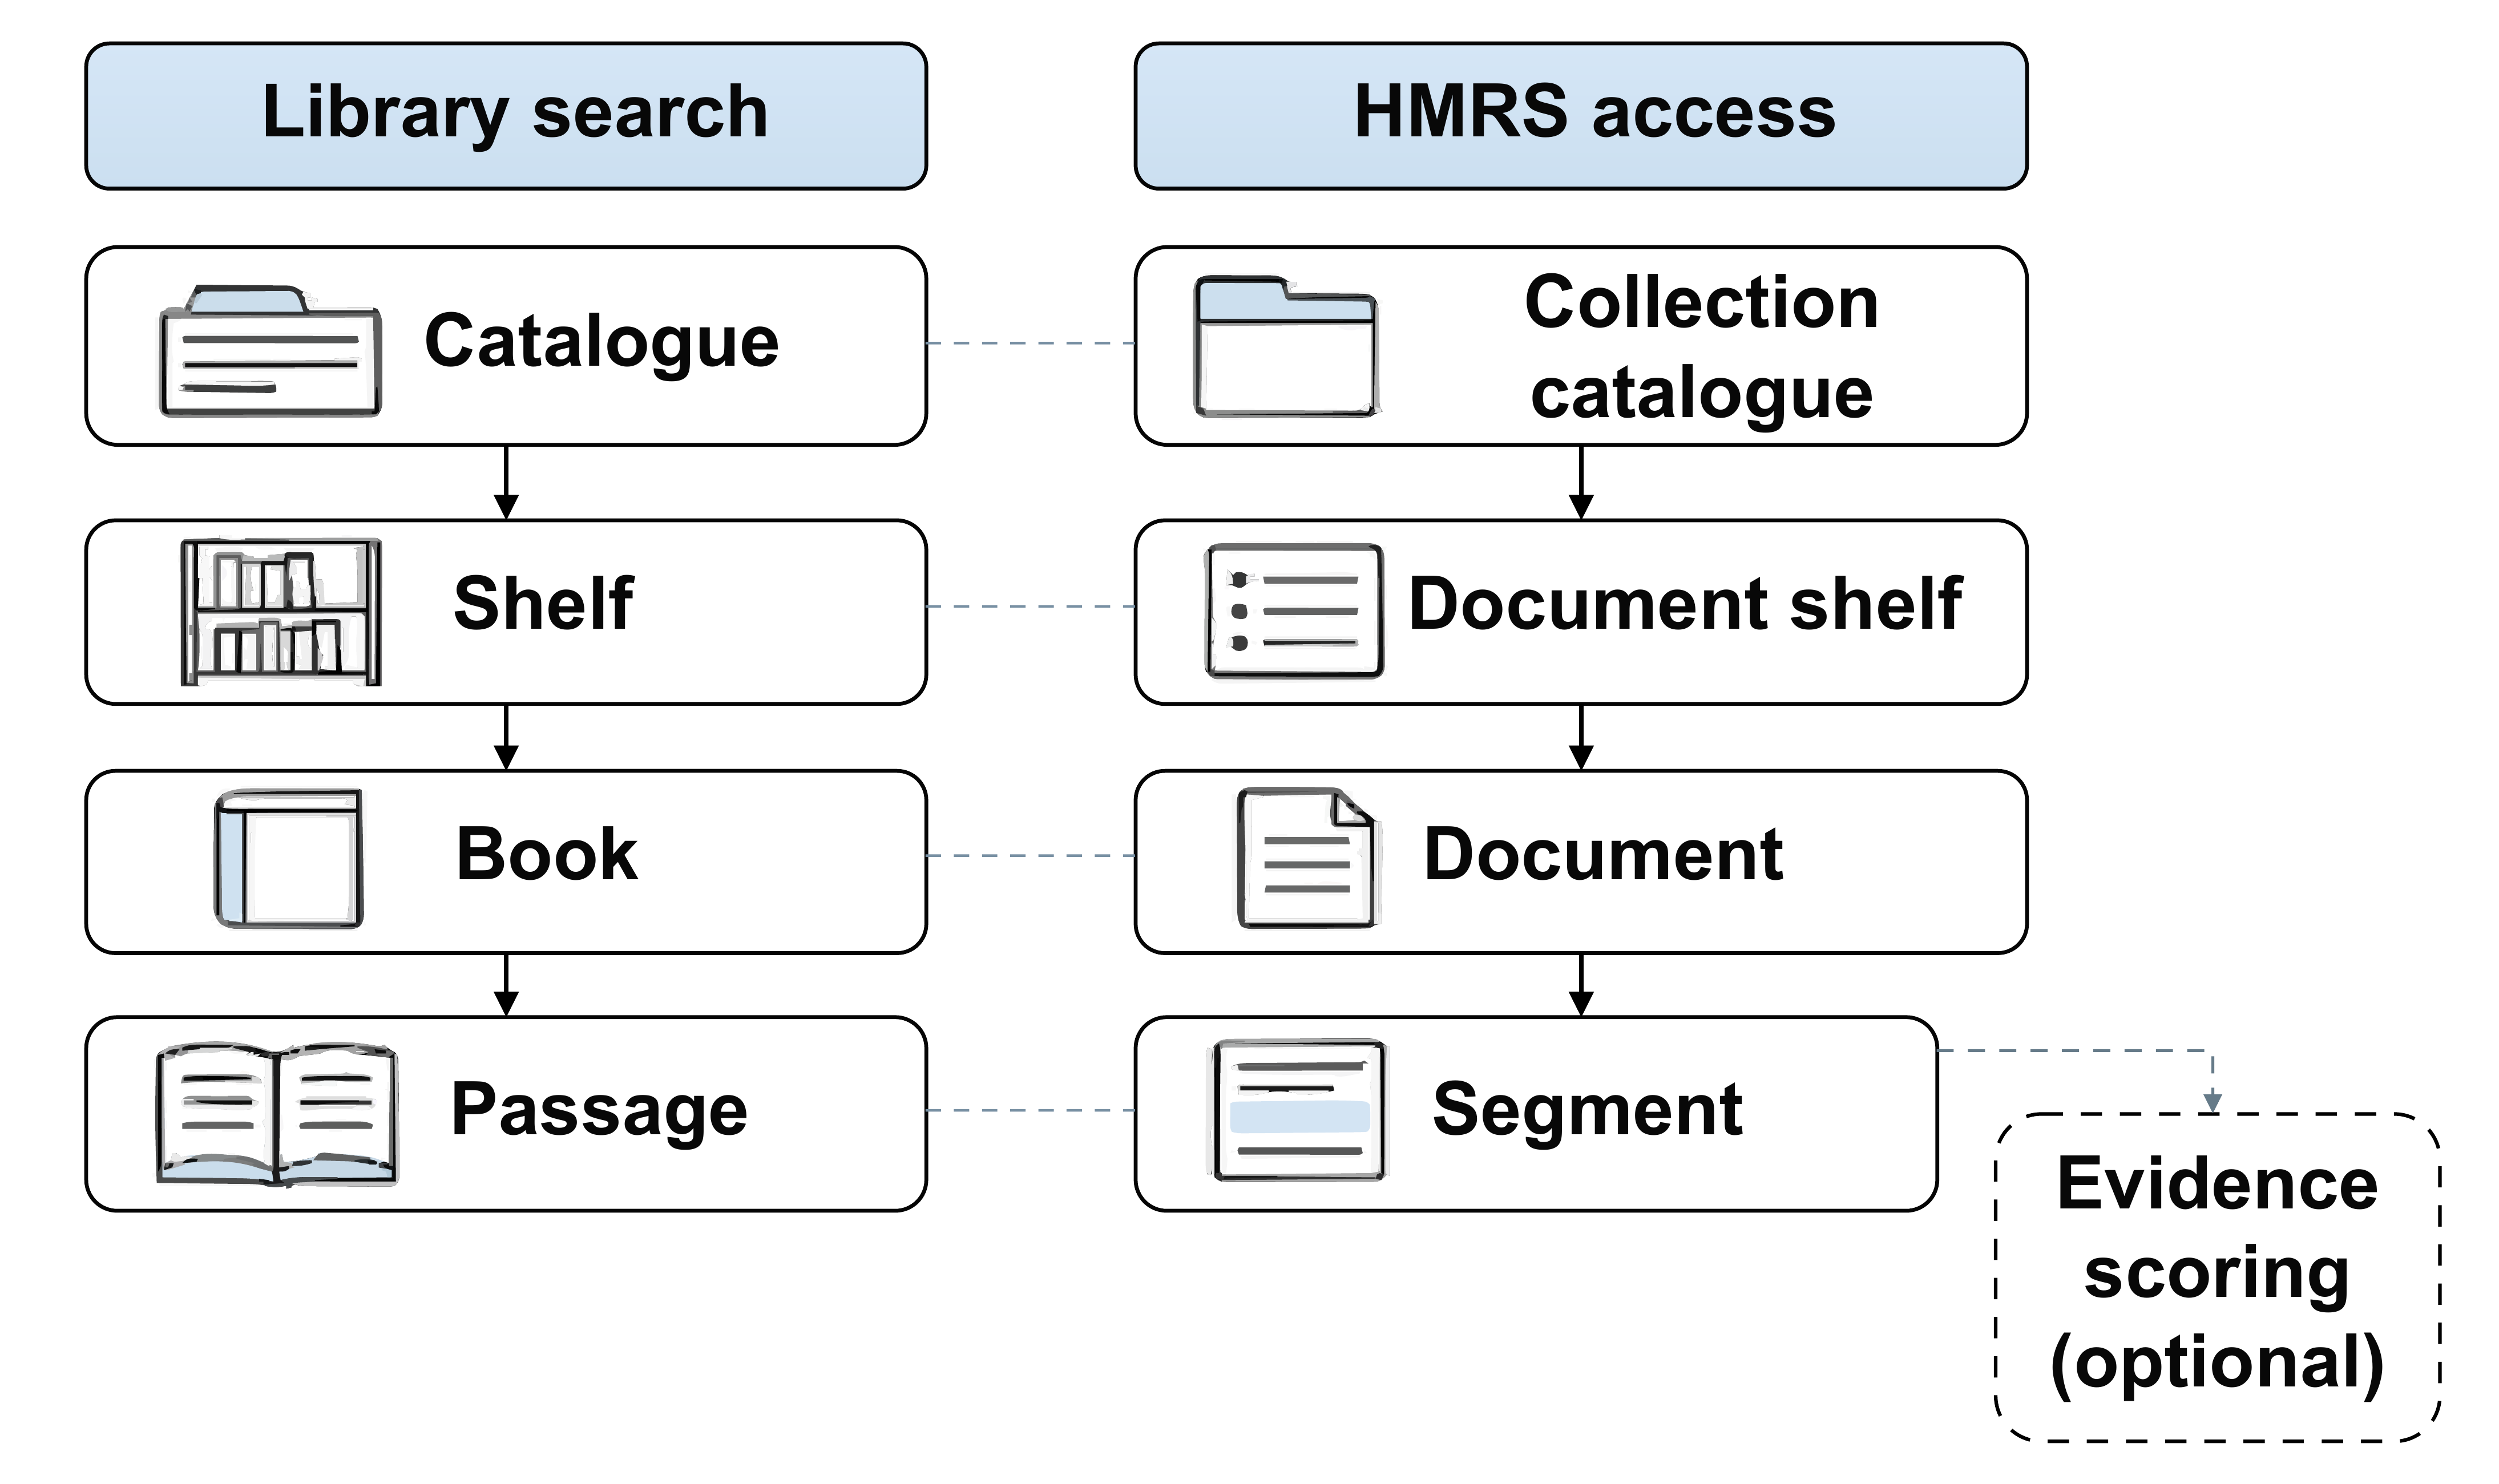
\includegraphics[width=4.1in]{figs/fig_library_analogy_vector.png}
\caption{\textbf{Figure 1.} Library analogy for a catalogue-first HMRS access path. The library catalogue, shelf, book and passage correspond to the collection catalogue, document listing, document body and segment. Evidence scoring is optional; pinned search may bypass the catalogue and shelf.}

\end{figure}

\setcounter{dbltopnumber}{1}
\begin{figure}
\centering
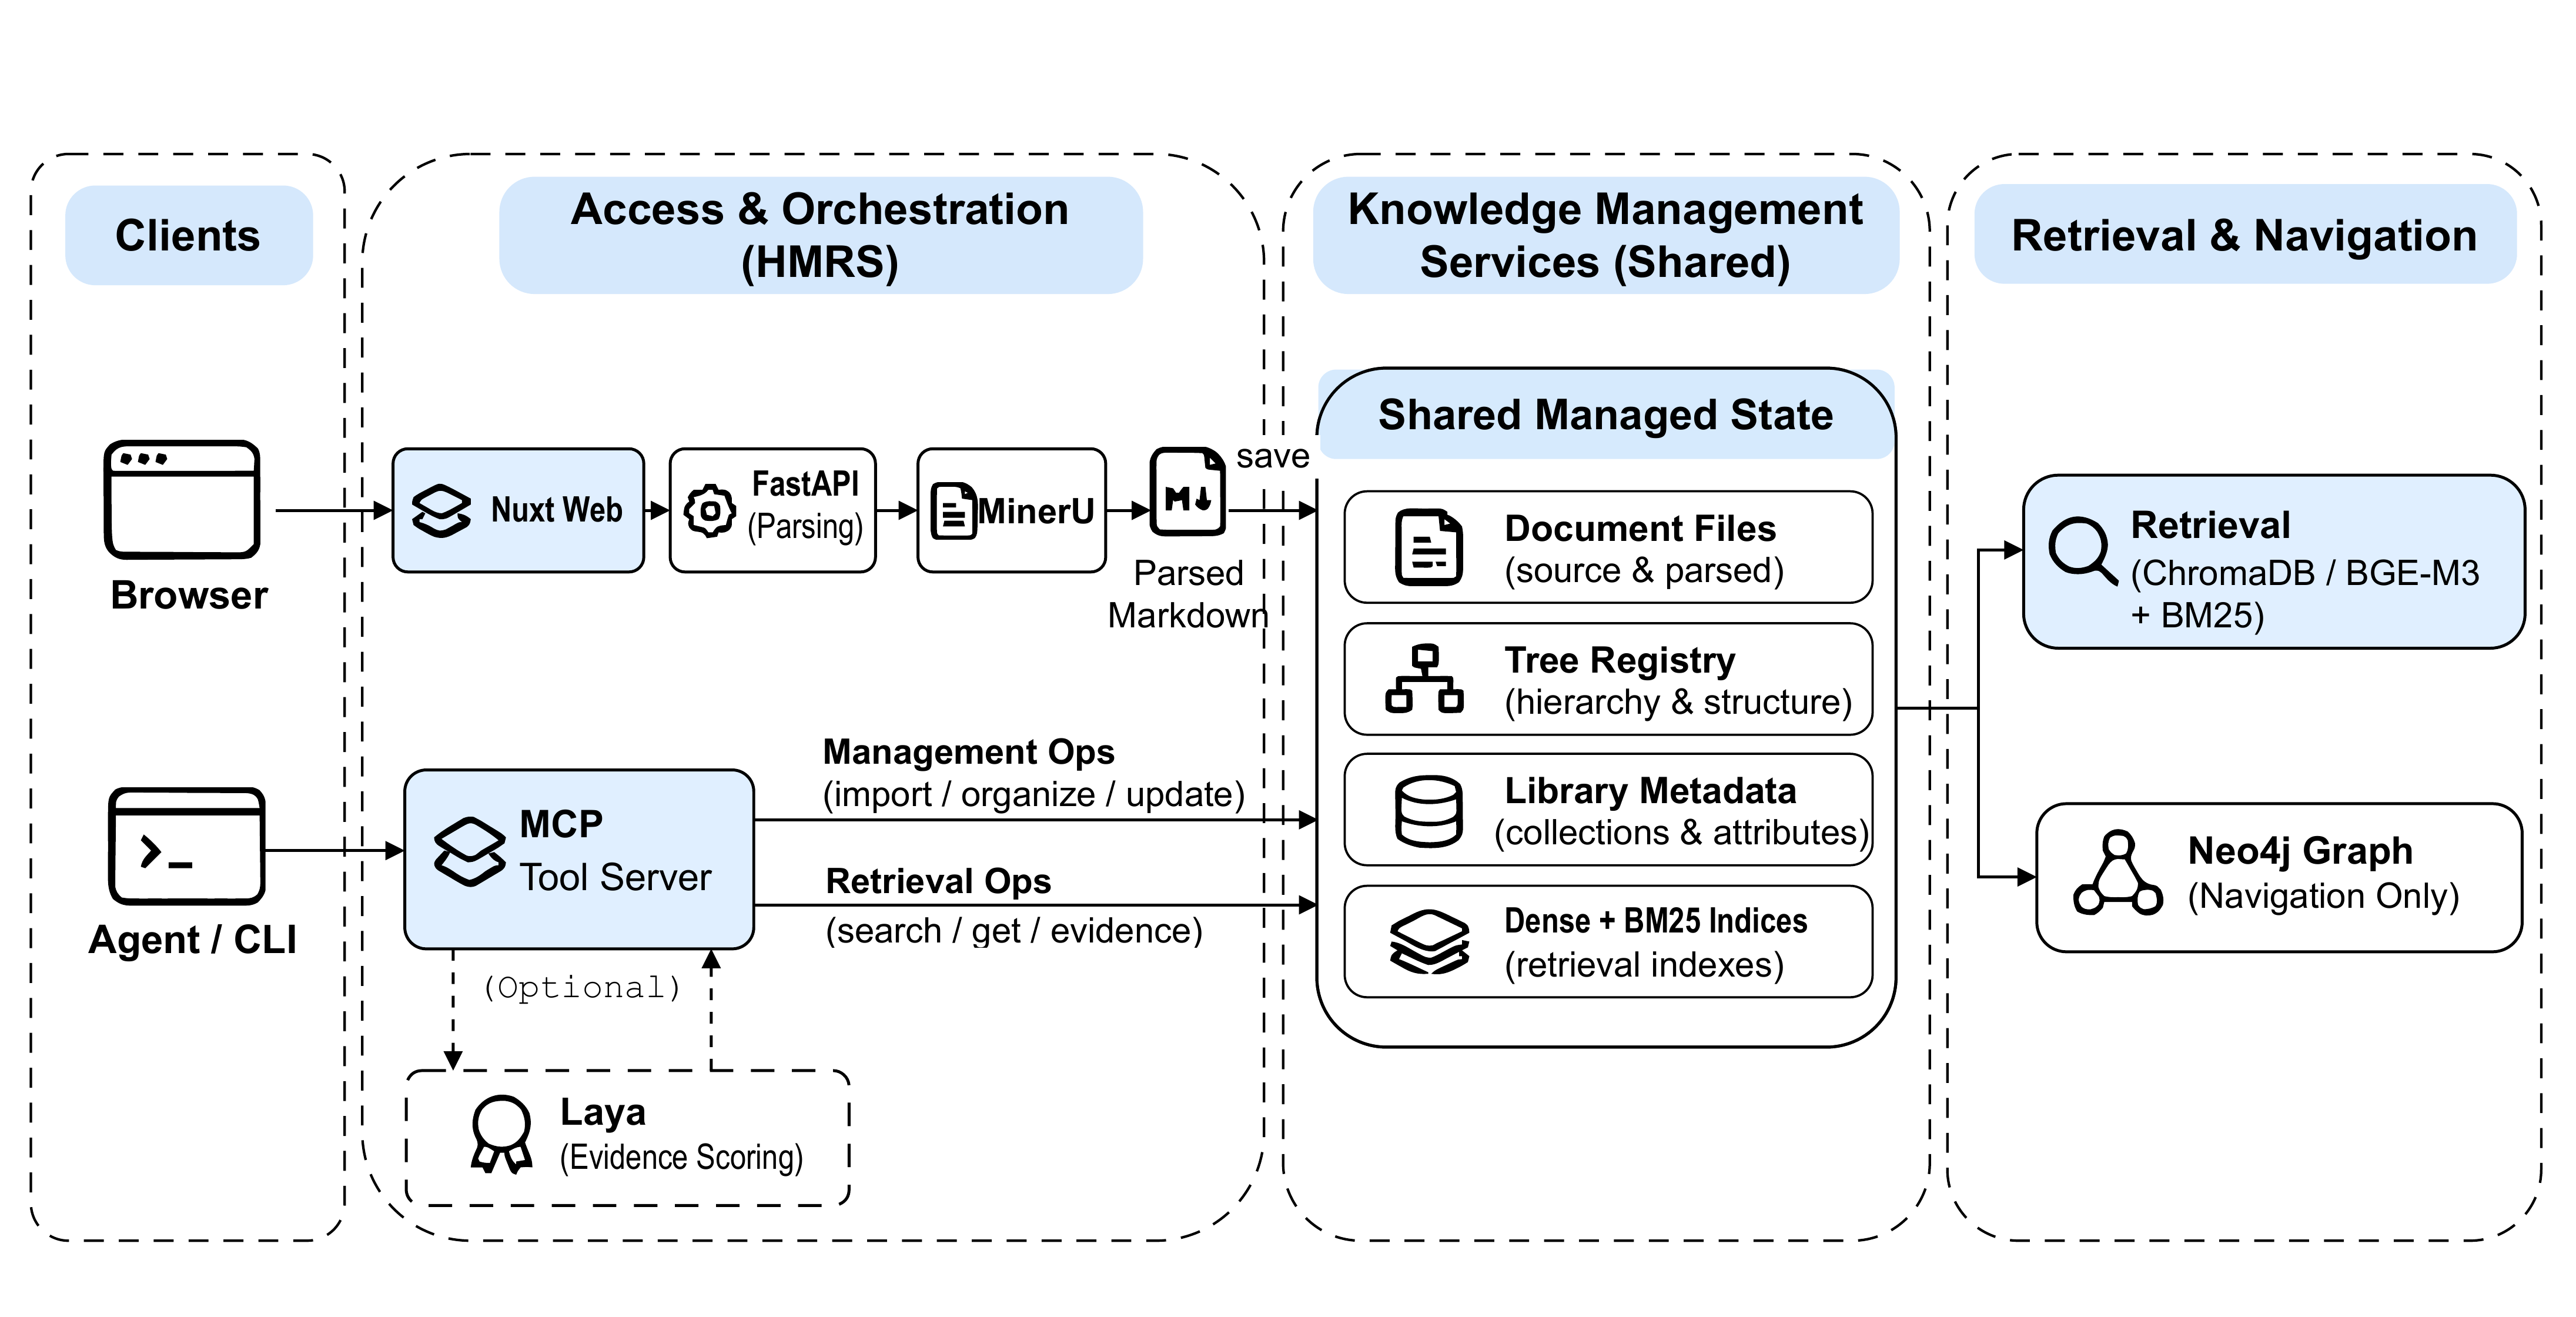
\includegraphics[width=6.45in]{figs/fig_service_architecture_vector.png}
\caption{\textbf{Figure 2.} HMRS service architecture. The browser and agent/CLI access the web and MCP interfaces. Parsing, management and retrieval operate on shared document files, the tree registry, library metadata and search indices. Laya scoring is optional, and the Neo4j graph supports navigation.}

\end{figure}

Figure~3 follows a document from acquisition and
organisation to evidence-based reporting. The ingest workflow governs
content review and placement. The query workflow determines whether to
consult the catalogue or search a pinned collection, and whether to use
Laya to score passages. The answer instructions distinguish a completed
review's searched scope and blind spots from an incomplete review caused
by tool failure.
Hybrid retrieval is also available as a tool and can be composed from
ordinary search calls. Experience retrieval and persona distillation reuse
the document infrastructure and define their own retrieval procedures.

Table~3 maps acquisition, organisation, lifecycle, query
and experience operations to the interface or workflow that checks them.
This allocation locates decisions at the appropriate boundary. For example,
the ingest agent chooses a collection, the save service validates the
destination identifier, and an audit checks the stored result.

\begin{table}
\centering
\small
\setlength{\tabcolsep}{4pt}
\caption{\textbf{Table 3.} Management functions, the enforcement or workflow check associated
with each, and the evaluation that exercises it. The table separates API/MCP
controls from agent procedures and campaign audits; semantic choices such as
which collection owns a document are made and recorded by the workflow.
Evidence labels E1--E9 denote the campaigns in Section~8.}

\begin{tabular}{@{}p{2.145cm}p{6.105cm}p{4.950cm}p{1.815cm}@{}}
\toprule
Group & Operations & Platform or workflow check & Evidence\\
\midrule
Acquisition & submit, parse (MinerU), quality review, duplicate review, structural split, store, index & parse-task state; workflow quality checks; entry-point-specific deduplication and indexing; post-index probe & E1--E2, S9\\
Organisation & create library or sub-library, content-informed placement, descriptions and tags, duplicate review & API validates identifiers and required fields; workflow checks descriptions and tags; audit compares files, tree and library metadata & E1--E2\\
Lifecycle & move, rename, delete, force re-index, graph build & operation-specific API updates; reconciliation audit detects selected stale or inconsistent state & E2\\
Query & tier selection, vector, keyword, catalogue and two-stage search, gate invocation & endpoint enforces tool allow/deny lists, timeouts and turn limits; invoked gate returns survivor provenance & E3, E5--E9\\
Experience & extract, approve, tier, search & experience tools apply their own retrieval, verification and credibility filters & E4\\
\bottomrule
\end{tabular}
\end{table}

\begin{figure}
\centering
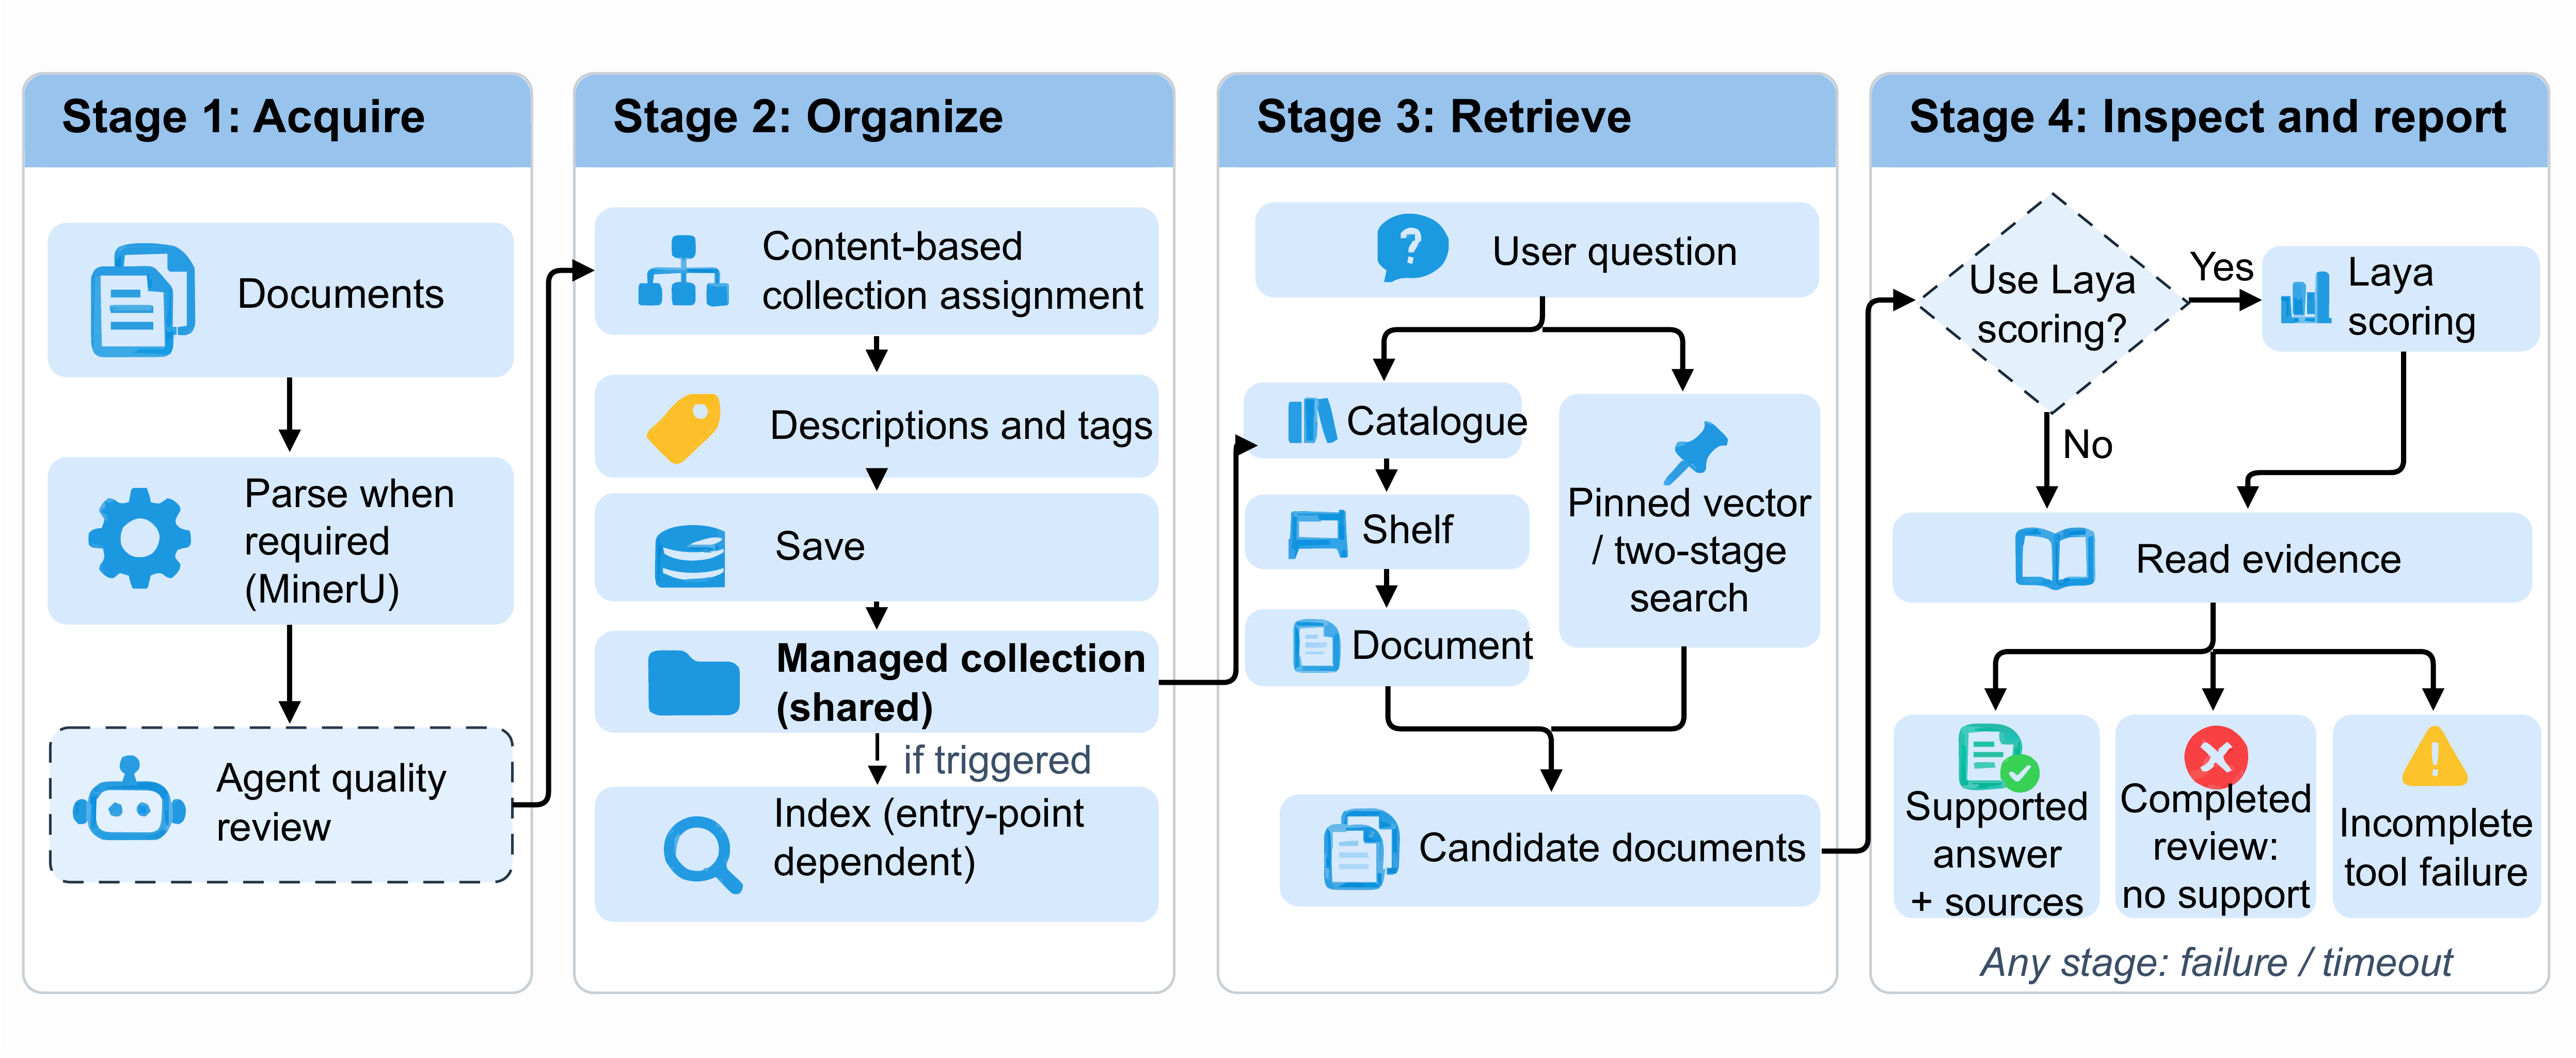
\includegraphics[width=6.45in]{figs/fig_workflow_vector.png}
\caption{\textbf{Figure 3.} Illustrative HMRS workflow from document acquisition to evidence-based reporting. Documents are parsed when needed, organised into collections and indexed according to the entry point. A question can use catalogue navigation or pinned search; optional Laya scoring precedes evidence inspection. A completed review without support is distinct from an incomplete search or tool failure, which may occur at any stage.}

\end{figure}

\subsection{3.2. Data model and object lifecycle}



Documents are stored as Markdown with associated assets. A managed
collection's state spans the document files, \texttt{.tree-fs.json} and the
library's \texttt{.knowledge-base.yml}. The ingest workflow distinguishes
parsed, stored and indexed content and records completion after a retrieval
probe. The MCP save path can start background indexing; the web parsed-file
save path exposes indexing as a separate operation. Reconciliation compares
the three representations and identifies selected stale-index conditions.
A move, rename or re-index can therefore be checked through the resulting
file path, metadata and retrieval response.


\section{4. Acquisition and automatic classification: from parsed document to
owned collection}


Acquisition establishes what a later search can find and where it can
look for it. HMRS parses PDFs, scanned images, Word and Excel files through
an asynchronous MinerU service [18]. The MCP parse tools return
pollable task identifiers. Markdown and plain text take the direct save
path. For parsed inputs, the ingest agent reviews the recovered body before
selecting a collection by topic.

The ingestion workflow connects parsing, review, optional splitting,
placement, storage and indexing. The source content informs the placement
decision, and the destination determines the scope of subsequent access.
The workflow records the applicable artefacts: a parse task identifier,
a quality report, a content fingerprint, a split manifest, a storage
record and the destination library. A content-based retrieval probe checks
that indexing exposes the document to later queries. This check follows the
save acknowledgement and tests a different transition.

\subsection{4.1. Quality gates and ingest lifecycle}

The upload service checks sibling files for exact duplicates using content
hashes. A separate near-duplicate tool returns pairs above a similarity
threshold for review. The ingest agent checks recovered text for OCR noise,
binary residue, missing section bodies, whitespace collapse and language
mismatch. It selects a library whose scope matches the recovered subject and
derives descriptions and tags from the same body. The owning collection and
its listing can then be checked after storage.

On oversized documents, the optional structural splitter groups recognised
units such as headings, Markdown tables, lists, block quotes and fenced code.
The research-paper campaign used a 30,000-character limit; later configurations used
60,000. The splitter aims to fill 85\% of the configured window and records
oversized indivisible units where applicable. Structure recognition covers
Markdown units, with formula-heavy pages depending on the quality of the
parsed representation.

The web parsed-file route persists Markdown and images. The MCP save tool
can also schedule vector and lexical indexing in the background. Graph
construction is a separate operation. Post-index checks can compare
expected identifiers with the recorded chunks and probe retrieval for
content from the saved document.

\subsection{4.2. Acquisition evidence and accounting limits}

The research-paper campaign provides an acquisition audit across five
libraries. Its target, indexed parts and observed retrieval coverage use
different units and are reported with their dates in Section~8.2.

In the separate multilingual ingestion test, a script sent 400 Wikipedia
pages per language to preassigned libraries. Their listings contained
87.5\% of expected English titles and all expected Chinese and Japanese
titles. This test checks listing coverage after a known placement decision.
Section~8.2 describes the listing and self-retrieval checks on the
same libraries.


\section{5. Collection and document management: organisation, classification and
lifecycle}


Collection membership defines the scope available to a query. HMRS uses
the subject of the content for placement, preserves the source assignment
across split parts, and exposes descriptions before an agent opens a
document body. The collection and document operations in
Table~2 maintain these choices over the life of the corpus.

\subsection{5.1. Classification, metadata, tags and duplicate review}





The catalogue returns collections and sub-libraries with descriptions.
Each shelf shows document titles and descriptions within its selected scope.
The ingest agent uses that scope and the parsed content to select a library,
then writes descriptions and tags grounded in the body. Duplicate review
presents candidate pairs for inspection because adjacent parts may share
metadata while retaining distinct source sections.

HMRS supports library and sub-library creation, metadata edits, moves,
renames, deletion and forced re-indexing. A move updates the document path
and registry entries, while re-indexing updates the searchable representation.
Integrity checks compare document existence, path and index metadata across
the files on disk, the \texttt{.tree-fs.json} registry and the library's
\texttt{.knowledge-base.yml}. These checks give operators observable
outcomes for the state changes made by each operation.

Sub-libraries keep their descriptions and indices at their own tree nodes.
When the caller supplies a parent scope, the vector service resolves the
parent and its descendants into the collections searched. The lexical stage
of the two-stage service likewise resolves descendant identifiers. The
tested flat union calls explicit library scopes, which fixes the collections
compared in the evaluation.

\subsection{5.2. Lifecycle operations, graph and operational knowledge}




A rename trial exposed a lifecycle defect: queries found chunks under the
old document path until a forced re-index. The current rename paths
synchronise the old and new index entries and record failures separately
from the metadata update. A post-operation probe can then check whether
queries resolve to the new path.

The document graph links libraries, documents and tags for navigation and
candidate expansion. Operational lessons are also stored as retrievable
documents. Experience tools track reviews, use and freshness and use
credibility tiers to order results. Section~8 reports
operational-experience cases alongside the management experiments.

\subsection{5.3. Organisation contract}



The organisation contract links each document to its current owning
collection, descriptive metadata and indexed path. The checks in
Section~8.3 test these relationships on selected lifecycle
operations by reconciling the three sources, reviewing document descriptions
and rerunning retrieval probes. The resulting traces locate inconsistencies
at the file, registry or index stage.


\section{6. The tiered access path: from collection to admitted segment}



A query reaches evidence by narrowing its scope. Catalogue-first search
selects a collection, examines the descriptions on its shelf and opens
selected documents or passages. Pinned search starts within specified
collections and uses their indices to propose candidates. Both paths can
call the server-side Laya evidence gate. This design gives an agent
explicit choices at collection, document and passage granularity and
preserves the source identifiers needed to inspect those choices.

Figure~4 and Algorithm~1 describe the
operations and terminal outcomes that an access policy can combine.
\begin{enumerate}
\item \emph{Rewrite.} Form search queries from the question.
\item \emph{Gather.} Select collection and document descriptions through the
catalogue or retrieve ranked candidates in a pinned scope.
\item \emph{Merge and cap.} Deduplicate multiple candidate sources and bound the
pool sent for inspection.
\item \emph{Score.} If requested, fetch reference text, score passages and
return survivors and their provenance.
\item \emph{Read and answer.} Inspect the evidence pack and open additional
source text as needed before answering with references.
\end{enumerate}

Access policies choose which operations to run. The intended workflow distinguishes
a completed review without support from an incomplete run with possible
partial evidence. This distinction depends on observable failure status;
the global-search defect in Section~8.10 shows it is not guaranteed
when a collection is silently skipped.

\begin{figure}
\centering
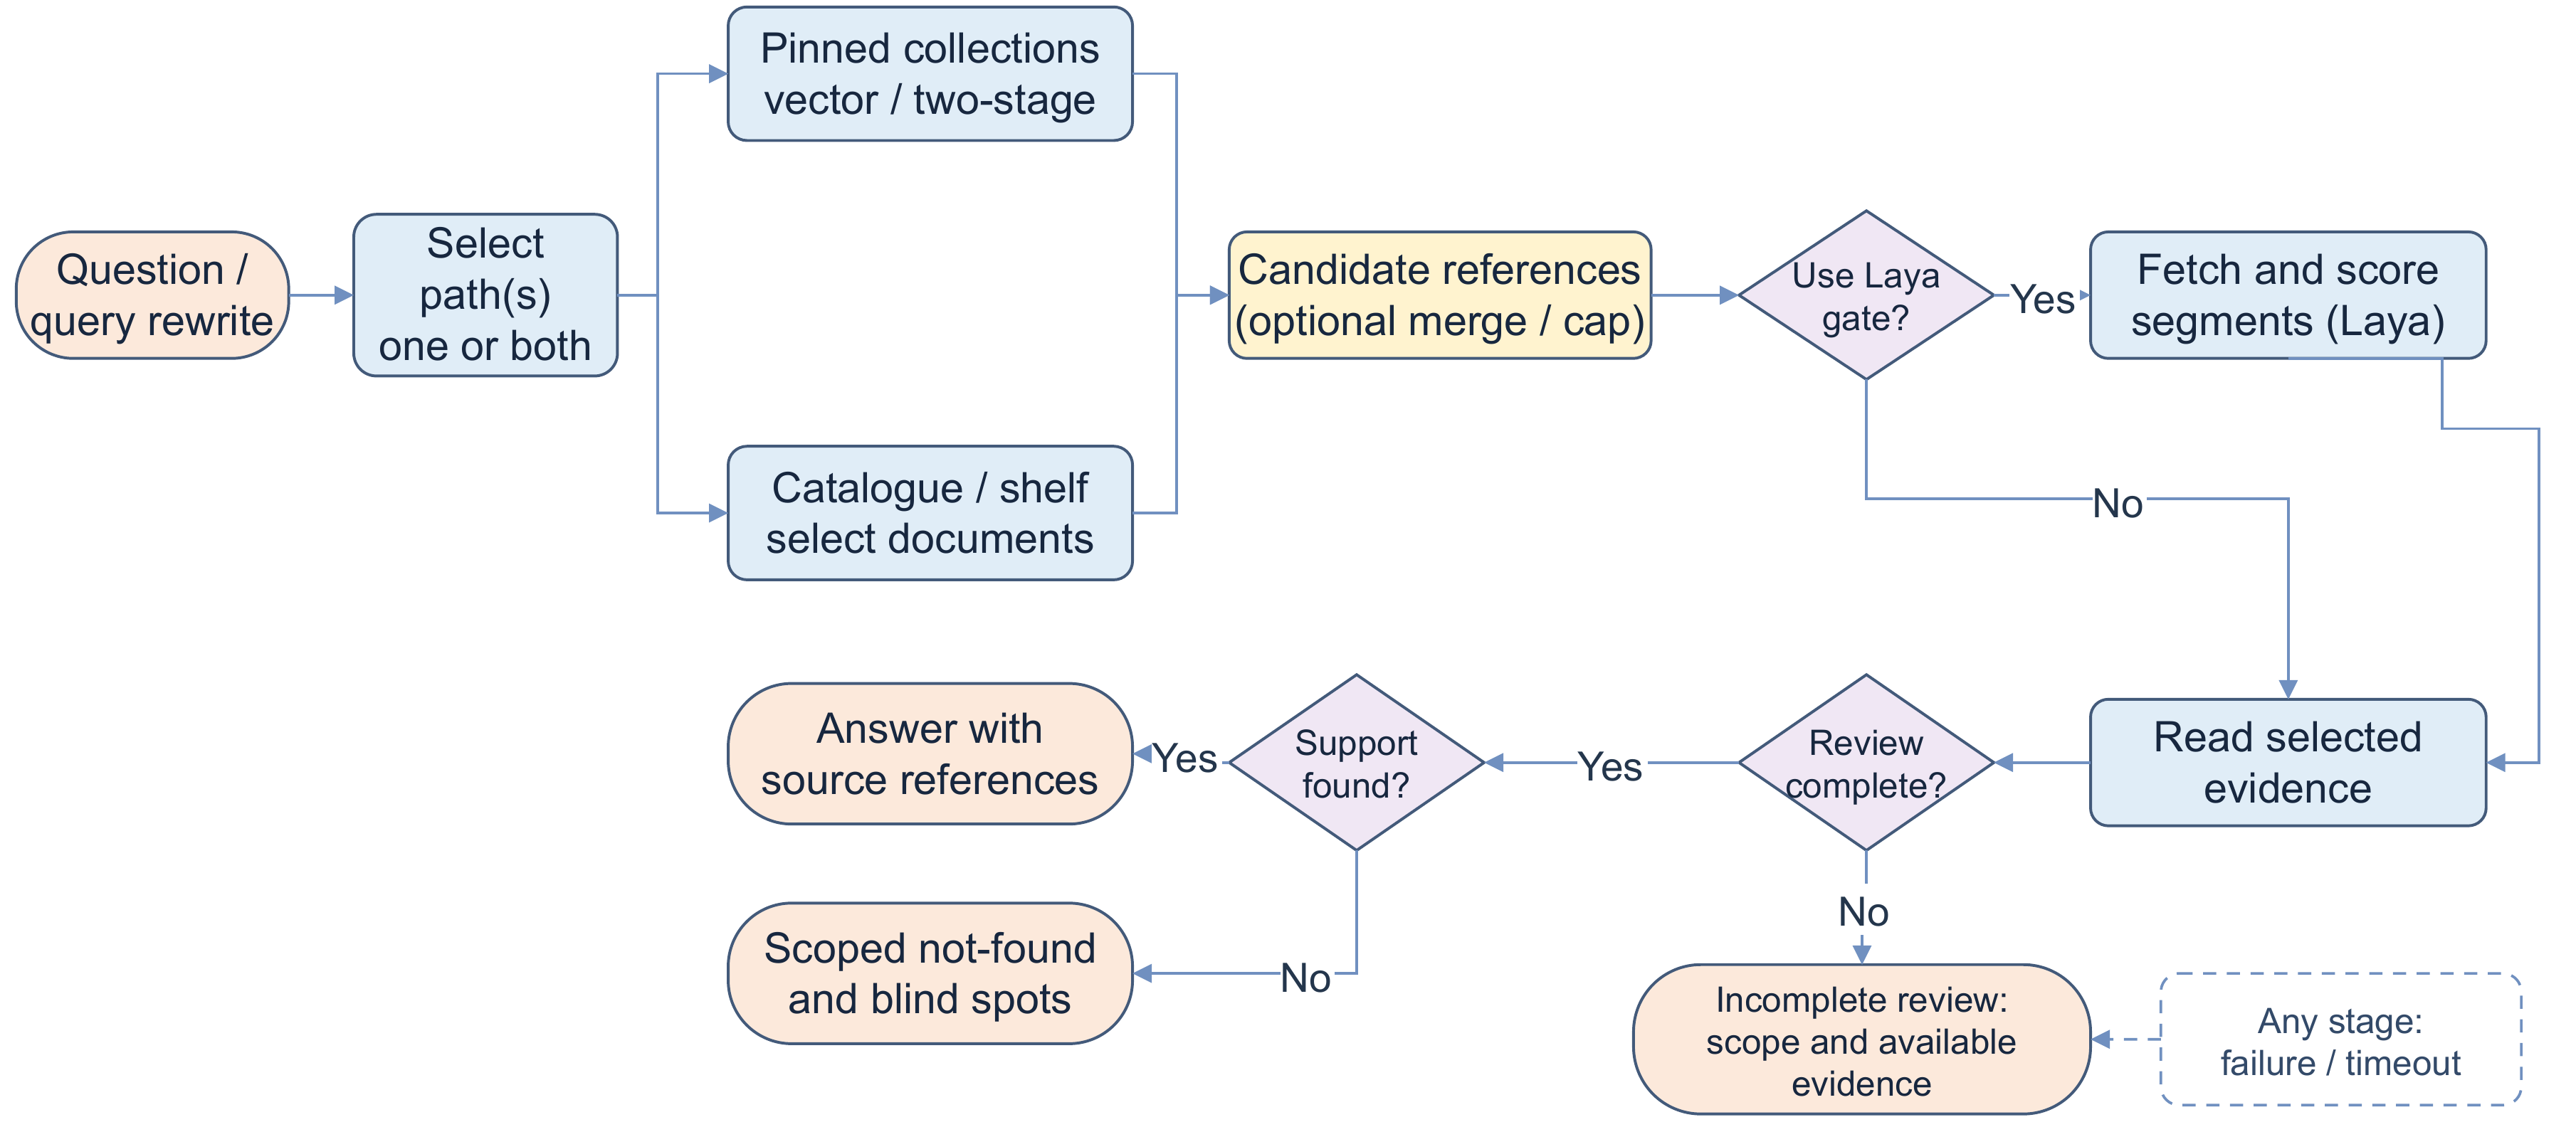
\includegraphics[width=6.45in]{figs/fig_tiered_drawio_20261116.png}
\caption{\textbf{Figure 4.} Tiered access workflow. Candidate references come from pinned
collections, catalogue navigation or a combination. The optional Laya gate
fetches and scores passages. A completed review without support reports
the searched scope. An incomplete operation reports failures and keeps
any available evidence.}

\end{figure}

\begin{quote}
\textbf{Algorithm 1. Tiered access with optional evidence gate}

\textbf{Require.} question $q$; catalogue $\mathcal{C}$; threshold $\tau$; gate flag $g$

1. $D \gets \mathrm{GatherCandidates}(q,\mathcal{C})$  (pinned or catalogue-first)

2. \textbf{if} $g$ \textbf{then}

3. $S \gets \mathrm{LayaJudge}(D,q,\tau)$  (fetch, score and return survivors)

4. \textbf{else}

5. $S \gets \mathrm{ReadSelected}(D)$

6. \textbf{end if}

7. \textbf{if} execution incomplete \textbf{then}

8. \textbf{return} incomplete status, searched scope, and available evidence

9. \textbf{else if} completed review finds no support \textbf{then}

10. \textbf{return} scoped not-found (searched scope, blind spots)

11. \textbf{else}

12. \textbf{return} agent-synthesised answer with source references

13. \textbf{end if}
\end{quote}
The policy instructs the agent to report its searched scope and remaining
blind spots when it reaches its call budget. The chat endpoint controls
timeouts and turn limits. Workflow instructions specify the retrieval
sequence and batch sizes.

\subsection{6.1. Tier policies and the evidence gate}





The knowledge-base chat interface defines two policies. The search policy
starts from pinned collections and calls two-stage or vector search. The
librarian policy starts from the all-library catalogue, uses shelf
descriptions to choose document references and directs the agent to score
them in sequential batches before reading the survivors. The two-stage
tool uses lexical search and optional graph expansion to form a candidate
pool, applies dense ranking and returns candidates for inspection.

The MCP server also registers \texttt{kb\_hybrid\_search}, which merges vector
and catalogue candidates, optionally applies Laya, and sorts retained
documents by verifier score when judging is enabled. The librarian policy
directs the agent to use the catalogue and shelf tools directly. A separate
controlled hybrid experiment used per-library vector top-30 at cosine
threshold 0.35, catalogue candidates, fusion and a cap of twelve. The
ordering analysis in Section~8.9 replays historical hybrid pools
to compare ways of using the recorded scores.

The local Laya classifier [62] is exposed as \texttt{kb\_laya\_judge}.
In reference mode it fetches candidate text, segments it and scores each
passage against the query. Passages whose \texttt{noul} score meets the
threshold (0.5 by default) are eligible for the returned evidence pack.
The gate orders survivors by source and position, deduplicates them and
applies a character limit. Its output carries provenance and separates
fetch or scoring errors from low scores, so a partial response can
retain successfully scored passages. The 0--1 score controls admission
to the pack. Candidate fusion and document ordering are separate
decisions that the calling workflow or hybrid tool applies. Laya scores
were used directly at the configured threshold, without calibration as
probabilities of entailment.

\begin{table}
\centering
\small
\setlength{\tabcolsep}{5pt}
\caption{\textbf{Table 4.} Access policies over the tiered path. Modes differ in how candidate collections and documents are selected.
The hybrid row describes the experimental composition used in the evaluation.}

\begin{tabular}{@{}p{1.815cm}p{3.135cm}p{3.960cm}p{2.640cm}p{3.300cm}@{}}
\toprule
Policy & Tiers traversed & Retrieval affordance & Budget type & Intended terminal report\\
\midrule
Search & pinned collections, segment & Two-stage or vector search & Endpoint turn limit & Answer or scoped not-found\\
Librarian & catalogue, shelf, document, segment & Catalogue navigation and passage scoring & Workflow instructions & Answer or searched scope\\
Hybrid & catalogue and segment & Combined vector and catalogue candidates & Configuration-specific candidate cap & Candidates or judged survivors\\
\bottomrule
\end{tabular}
\end{table}

Response transport also determines which candidates the agent can see.
The 13 October catalogue incident exposed truncation before the agent
could inspect the whole shelf. The shelf tool now caps its response and
supplies grouped and paginated views, allowing the caller to request the
remaining entries. Section~8 reports the repair check.

\subsection{6.2. Honest abstention}
The answer workflow asks the agent to report absence after a completed
review that finds no support, including the scope it searched. A plausible
candidate may still lack the required evidence. If a tool is unavailable
or the search times out, the workflow reports the incomplete execution
and any usable evidence. Section~8 reports how the agents
handled these terminal conditions in the observed trials.


\section{7. Agent interface and implementation}



\subsection{7.1. MCP tools and lane policy}


MCP exposes the management groups in Table~3 to agent
harnesses. Long-running parsing, forced re-indexing and graph construction
return task identifiers that a caller can poll. Catalogue, document read,
search and passage-scoring operations expose different views of the
resulting state. An operator can verify a write by probing its resulting
collection and document paths, then re-index if needed. Figure~S1 shows the tool layer and
its management and retrieval services.

The knowledge-base chat endpoint mounts the MCP server and supplies
read-oriented tool sets. Administrative writes use management tools and
their own permissions. The endpoint sets time and turn limits, while the
policy instructions direct the retrieval sequence and set batch sizes.
A separate KB agent endpoint adapts multiple harnesses for management and
other knowledge-base tasks and supports asynchronous task execution.
Persona distillation uses the same storage infrastructure with its own
retrieval and synthesis path.

\subsection{7.2. Runtime and deployment}


The backend uses Python 3.12 and FastAPI. ChromaDB stores cosine-space HNSW
collections with normalised 1024-dimensional BGE-M3 embeddings
[63, 64, 35]. BM25 supports lexical search [32], Neo4j
stores the document graph [65] and MinerU provides parsing and OCR
[18]. The local Laya worker queues scoring jobs to serialise GPU
execution.

The experiments ran on one self-hosted Windows workstation with an RTX
5060 GPU (8 GB) for embeddings and scoring. A stack recovery script checks
the API, web and MCP services and starts missing processes before evaluation
probes. In three acceptance trials the script restored a stopped stack
without manual intervention.

The implementation and scripts are available at
\url{https://github.com/kingdol666/rag-knowledge}. Use of the experimental
corpora remains subject to their data-use constraints.


\section{8. Evaluation}

The evaluation follows a document from ingestion and organisation to
retrieval and use. E1, E2 and E4 test the managed state and its lifecycle
(RQ1). E3 tests whether catalogue routing selects the intended collection
(RQ2), and E5 measures what each retrieval configuration puts into its
evidence pack (RQ2--RQ3). E8 tests how verifier-based ordering changes the
top five (RQ4). E6 and E7 examine answer traces, refusals and execution
costs (RQ5), and E9 reports operational checks across the workflow.
Tables~S9--S10 and S17 record the protocols and provenance.

\subsection{8.1. Experimental design and measures}


\textbf{Corpora and questions.} The industrial corpus contains 42 documents
in five libraries, including twenty near-duplicate telemetry reports. It
has 16 questions with annotated document fragments. Q16 shares a token with
its gold filename. A research-paper campaign sampled 100 papers from arXiv
across about 25 domains; ten questions have gold papers annotated by their
source identifiers, which are absent from the saved question texts.
A November
metadata recheck enumerated 328 parts in five libraries, including six parts
from non-target documents. The
cross-lingual campaign used 400 Wikipedia pages and 40 extractive queries per
language (English, Chinese and Japanese). Its ingestion script placed pages
in predefined language libraries and checked the resulting listings.
The routing and content benchmark used 138 documents stored as 879 parts in
ten domains and 72 in-domain questions. The released traces for complete
arms also contain four out-of-domain probes (R1--R4), reported separately.
The benchmark excludes the two cross-domain placeholders X1 and X2. The
follow-up used the same 72 questions after the corpus grew to 906 parts.
The questions and gold annotations were developer-authored. A post-hoc
check lowercased each question and its nonempty annotated target string,
then tested whether the entire target was a substring of the question,
without other normalization. This identified overlap in 29 of 72 questions;
the remaining 43 did not match under this test. The check describes the
questions and does not rescore the returned packs.

\textbf{Measures and controls.} Document-level Hit@5, Recall@5 and
MRR@5 are evaluated on the five returned documents, with reciprocal rank set
to zero when the top five contain no gold item [66].
The route check tests whether the script selected the labelled collection.
Target-string containment records whether the annotated string occurs
anywhere in the returned evidence pack, including in a sibling document.
The answer grids check for a gold paper identifier in the answer or trace,
for at least $\lceil 3n/5\rceil$ of $n$ annotated terms (strict matches or,
in the alias-aware check, accepted variants), and for a document-style
citation marker. These lexical checks measure the presence of expected
text and citation formatting. Semantic assessment and graded relevance
would require distinct criteria, as in RAG evaluation frameworks
[67, 68] and cumulated-gain measures
[69].

Wilson intervals describe the observed question sets. Paired exact
McNemar tests are two-sided and exploratory, with unadjusted $p$ values.
Each agent arm used one model and one run per condition, with transport
retries treated as part of that run. The answer grids used the platform chat
API with the Claude Code engine. A separate four-question case compared
Claude Code with oh-my-pi using \texttt{ustc/deepseek-flash} in November
2026. Two corpus-integrity defects were repaired before measurement.

\subsection{8.2. E1: Acquisition and parsing}

The campaign targeted 100 papers. In the November 14--15 disk inventory,
every target had at least one stored part; the five libraries contained 328
parts in total, including six from non-target documents. All 328 had
metadata descriptions of at least 60 characters without the recorded
placeholder pattern. This establishes neither complete paper coverage nor
retrieval quality.

Earlier records report 91 names in an ingest-state list and 79 documents
enumerated and read from a derived library. These are not matched target
sets or stages of a 100-paper funnel, and the records do not establish a
reliable date or individual failure stages. An initial November probe also
recorded misses. After forced reindexing, explicit indexing and a probe-tool
correction, a filename-stem short-query diagnostic found all 100 target
identifiers in returned names. However, 72 searches were unrestricted by
library and 45 returned a chunk-copy name first; this is not a matched
before--after retrieval comparison. A ten-question vector check restricted to
the five libraries placed the gold document first and invoked the judge in
all ten cases. The retained summary covers initial retrieval, with
incomplete records for the judge inputs and final evidence packs.

The Wikipedia ingestion check found 350 of 400 expected titles in the
preassigned English library and 400 of 400 in each of the Chinese and
Japanese libraries. Its separate self-retrieval check used the first
three index results. These tests exercise document placement and
index access for known inputs. In a 50-paper campaign spanning 26
domains, all 50 papers passed the parsing and verification checks.
The run recorded 41 negative tag flags without blocking ingestion.

\subsection{8.3. E2: Organisation, consistency, and management operations}

A rename in a test library exposed stale index state. The index returned
18 chunks where nine were expected, producing duplicate results. Forced
reindexing restored the expected nine. A separate five-library inventory
recorded 322 parts; its archived content snippets were nonempty for all
322, but retained at most the first 1,000 characters per part. A 33-part
sample passed checks across files, tree entries and
library metadata. A three-level
test library supported parent-to-child moves, listing, reading and
judging. Of the 16 lifecycle scenarios, the create, move, delete and
forced reindex checks passed, and the task-status and update checks
failed. The campaign left merge and split outside the controlled tests.

Near-duplicate review flagged 35 candidate groups at a threshold of~0.90
(scores 0.90--0.975). Review found no true duplicates and removed no
documents (Table~S9). The tag check passed 165 parts and exposed orphan
tags and one cross-library registry leak. A document move in the 658-node
graph added four tag edges (4,675 to 4,679), recording the change in the
navigation view.

\subsection{8.4. E3: Paired route-card audit: the description-layer contrast}

The script selected the labelled collection for all 72 in-domain
questions using description-bearing route cards (A0), and for 37 using
nominally name-only cards (A3). The 35 changed decisions all favoured A0
(Figure~5a, exact McNemar $p=5.82\times10^{-11}$). The
design compares the two route-card configurations. A3 could fall back
to descriptions without logging the fallback, some questions share
titles with the descriptions, and A3 can search outside the evaluation
scope. Among the 72 questions, 52 were expanded automatically, and
47 came from three domains.

Selecting the correct collection left a separate evidence-selection
problem. The returned packs contained the target string in 37 A0 and
33 A3 cases (10 A0-only, six A3-only, $p=0.4545$). The mechanical full
scan located all 72 targets (Figure~5b), including the
35 missed by A0 ($p=5.82\times10^{-11}$). It issued 64{,}584 tool calls
across these questions, averaging 897 calls and 24.3 MB of recorded text
per question. The containment--text-volume plot in
Figure~5c shows the cost of this reference point.
Section~8.6 compares the evidence packs across
retrieval configurations.

\begin{figure}
\centering
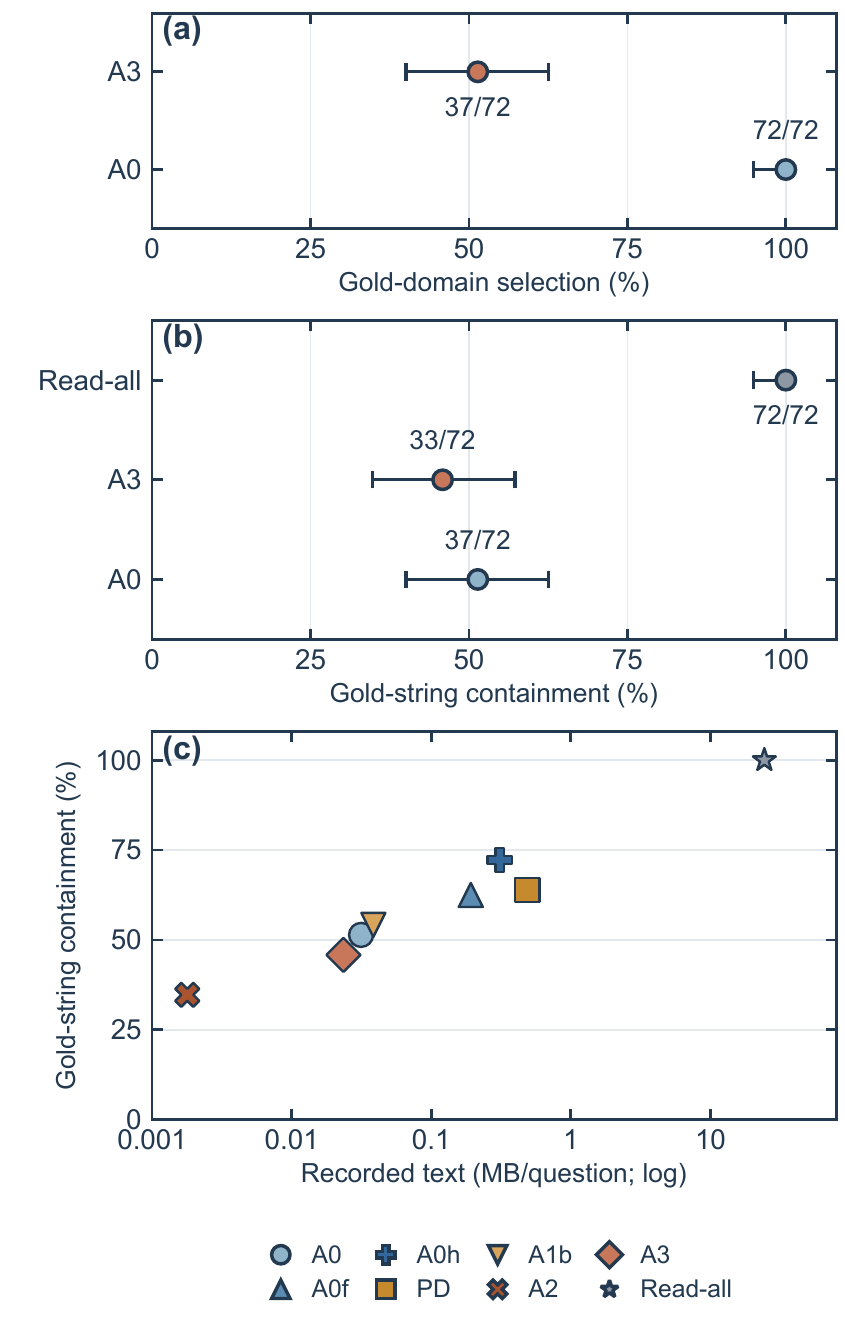
\includegraphics[width=4.1in]{figs/fig_opt_route.png}
\caption{\textbf{Figure 5.} Route-card and evidence-pack diagnostics on 72 in-domain
questions. (a) Labelled-collection selection with Wilson 95\% intervals.
(b) Annotated target-string containment in returned text. The read-all
arm performs a mechanical substring scan and generates no answers.
(c) Frozen trace-recorded text per question (MB, log scale) and
containment. The A0f and PD markers are offset horizontally by 8~pt
for legibility. The source data retain their original coordinates.
Recorded text and tool time measure the retrieval work in the trace.}

\end{figure}


\subsection{8.5. E4: Operational knowledge and automated distillation}

HMRS stores operational lessons as searchable documents and uses a
credibility tier to decide which lessons to present
(Section~5.2). A script-driven heuristic smoke test
reported 13 draft lessons from one small library. A separate case report
states that one lesson (\texttt{exp-d6f4d47ae3d6}) was stored and ranked
first by global experience search, but the original successful response
was not located, so this is a report-level observation. An approval check
found the draft pool empty on that occasion, and a heuristic dry run
produced output that failed the quality criteria. These limited checks do
not establish performance at scale. Scheduled distillation, review and
approval at scale, application feedback and credibility decay remain
untested.

\subsection{8.6. E5: Content-layer configuration comparison}

A0 selects a collection from the route cards and gives candidate references
to a judge with a 40{,}000-character document window. A0f fetches windows of
up to 250{,}000 characters and passes them directly to the judge. A0h
combines the resulting judged text with up to eight vector-retrieved chunk
windows in a pack capped at 60{,}000 characters. PD searches the ten libraries
separately and judges the six unique documents with the highest scores using
the A0f window. A1b merges the ten libraries' vector results and uses the A0
reference-mode judge. A2 concatenates snippets from the same scoped union
and omits judging. A3 uses the nominally name-only route cards. Within the
routed library, vector search requests up to 30 candidates at a cosine
threshold of 0.35, with a retry at 0.30 if the first search is empty.
The configurations vary in routing, candidate construction and judging.
Some reference lookups may use the gold domain to resolve candidates,
as detailed in Section~10.

\textbf{A0h contained more target strings than the other bounded-pack
configurations in the latest complete seven-arm trace.} On November~17,
A0h contained 48 of 72 targets (66.7\%, Wilson 95\% interval
55.2--76.5\%), compared with 36 of 72 (50.0\%) for A0. The difference
was 16.7 percentage points: 12 questions favoured A0h and none favoured
A0 (two-sided exact McNemar $p=0.00049$, unadjusted). PD contained 42
targets, A0f 41, A1b 36, A3 26 and A2 23. This rerun used the
restarted live stack; read-all was not rerun.

The earlier frozen record contained 52 targets for A0h and 37 for A0,
a 20.8-point difference with 15 A0h-only hits and no reverse cases
($p=6.1\times10^{-5}$). In the November~12 follow-up, the corresponding
counts were 51 and 39, with 12 A0h-only hits ($p=0.00049$). Across the
frozen and follow-up records, PD contained 46 and 45 targets, A0f 45
and 44, A1b 39 in each, and A2 25 in each. Figure~7 shows
these historical records, not the November~17 trace; Table~S12 lists all
three campaigns separately.

The following diagnostics refer to the frozen and November~12 records.
The paired comparison with the scoped vector union A1b favoured A0h on
13 frozen and 12 follow-up questions, with no reverse cases
($p=0.00024$ and $0.00049$). A0h's lead over PD was smaller. In both
records, seven questions favoured A0h and one favoured PD
($p=0.0703$). Among A0's 35 frozen misses, A0f, A0h and PD recovered
8, 15 and 9, respectively. Eight recoveries were shared by all three,
seven were unique to A0h and one to PD. Nineteen were missed by all three.
A post-hoc search placed five first matching occurrences outside the
nominal window and 30 inside. The matching file could differ from the gold
document or the one the judge read. Figure~7b and Table~S13
give the paired records, including the secondary comparisons.

The historical frozen A0h trace recorded 309~KB and 13.8~s of tool time per question, compared with
31.4~KB and 16.3~s for A0. The frozen read-all scan found all 72 target strings
using 24.3~MB and 253.7~s per question, about 79 times the text recorded
for frozen A0h; it is not a measurement from the November~17 run. The trace
counts overlap where the same text is fetched or packed more than once. Tool
time covers retrieval work and excludes answer generation. In the November~12
follow-up, the A0 tool-time median was 9.8~s (mean 17.4~s, maximum 540.9~s).
The separately executed A3 follow-up contained 25 target strings, down from
33 in the frozen record, and selected the gold domain on 49 questions. It
returned no top candidate in 13 cases and an empty pack in 23. The follow-up
read-all merged trace contains only three rows; its checkpoint contains 16
unique completed in-domain rows, all hits. The scan remains incomplete and
is excluded from the 72-question comparison.

An independent response-capture reproduction of the four content arms
matched the frozen hit status on 71/72 questions for A0f, A0h and PD and
on 68/72 for A0; its hit/miss records match the November~12 follow-up for
these arms. A1b and A2 also had identical frozen and follow-up hit sets.
In the November~17 trace, all three \texttt{F-hlm} questions were missed
by A0, A0f and A0h despite correct routing: each recorded an empty top
candidate, no survivors and an empty pack. The cause of the empty candidates
is undetermined. Corpus state was not held fixed across runs, and the trace
comparison does not establish verbatim reproducibility of response text.

In a separate 40-question diagnostic, the returned text contained the target
in 24 BM25 cases, 19 dense-search cases and 26 cases when the top five
texts from each list were concatenated. This check used different
questions, scopes and evidence construction. The trace label
\texttt{F-rrf} denotes concatenated lists.

Figure~6 shows two evidence paths from the independent
November~11 response-capture reproduction, not frozen-run response texts.
For the five case-arm paths displayed, the capture's containment flags agree
with the frozen trace; this agreement is not a claim about other questions.
For the question on RoBERTa, the captured A0h pack contains a passage mentioning
RoBERTa in Lewis et~al.'s RAG paper, a different document from the
annotated source. For the \emph{Pride and Prejudice} question, captured A0's top
candidate is part~2, but its sole survivor is part~6; captured A0f's survivors are
parts~21 and~6. Neither captured response contains the exact target string. A0h
includes the requested opening dialogue in part~2, but a line break splits
the target phrase there. Its contiguous exact match occurs instead in a
later dialogue in part~24. The recorded HIT therefore reflects string
containment, not verification of the requested context or answer correctness.

\begin{figure}
\centering
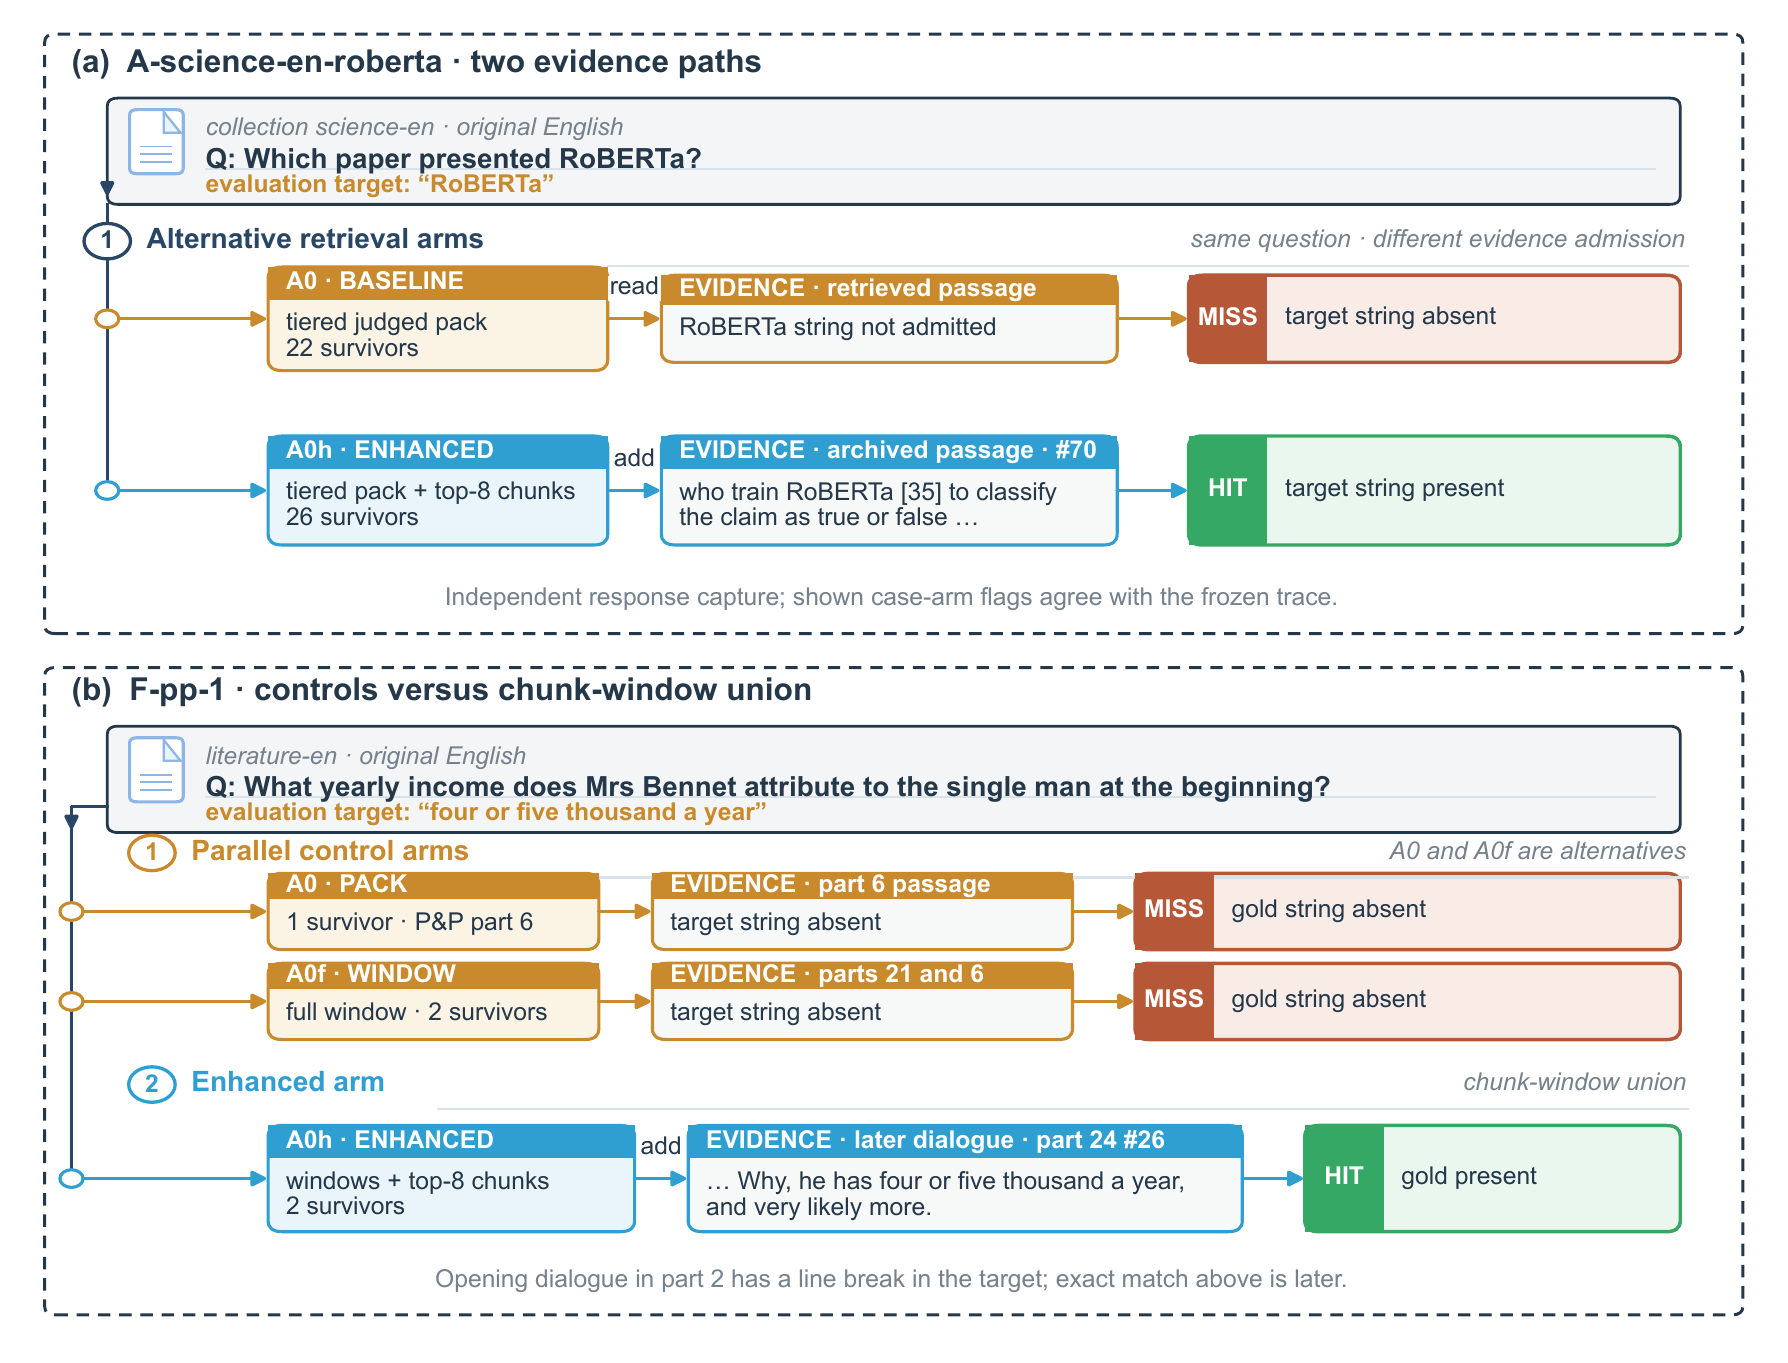
\includegraphics[width=6.45in]{figs/fig_opt_case.png}
\caption{\textbf{Figure 6.} Evidence paths from an independent November~11 response-capture
reproduction, not frozen-run response texts. The five displayed case-arm
containment flags agree with the frozen trace. (a) A0h includes a passage
containing \emph{RoBERTa} in the paper by Lewis et~al.~[7].
The bracketed reference in the excerpt uses the source paper's numbering.
(b) A0h's exact match for \emph{four or five thousand a year} occurs in
later dialogue (part~24); its opening dialogue (part~2) splits the phrase
across a line break. HIT and MISS refer to exact target-string containment
in the captured pack, not answer correctness.}

\end{figure}

\begin{figure}
\centering
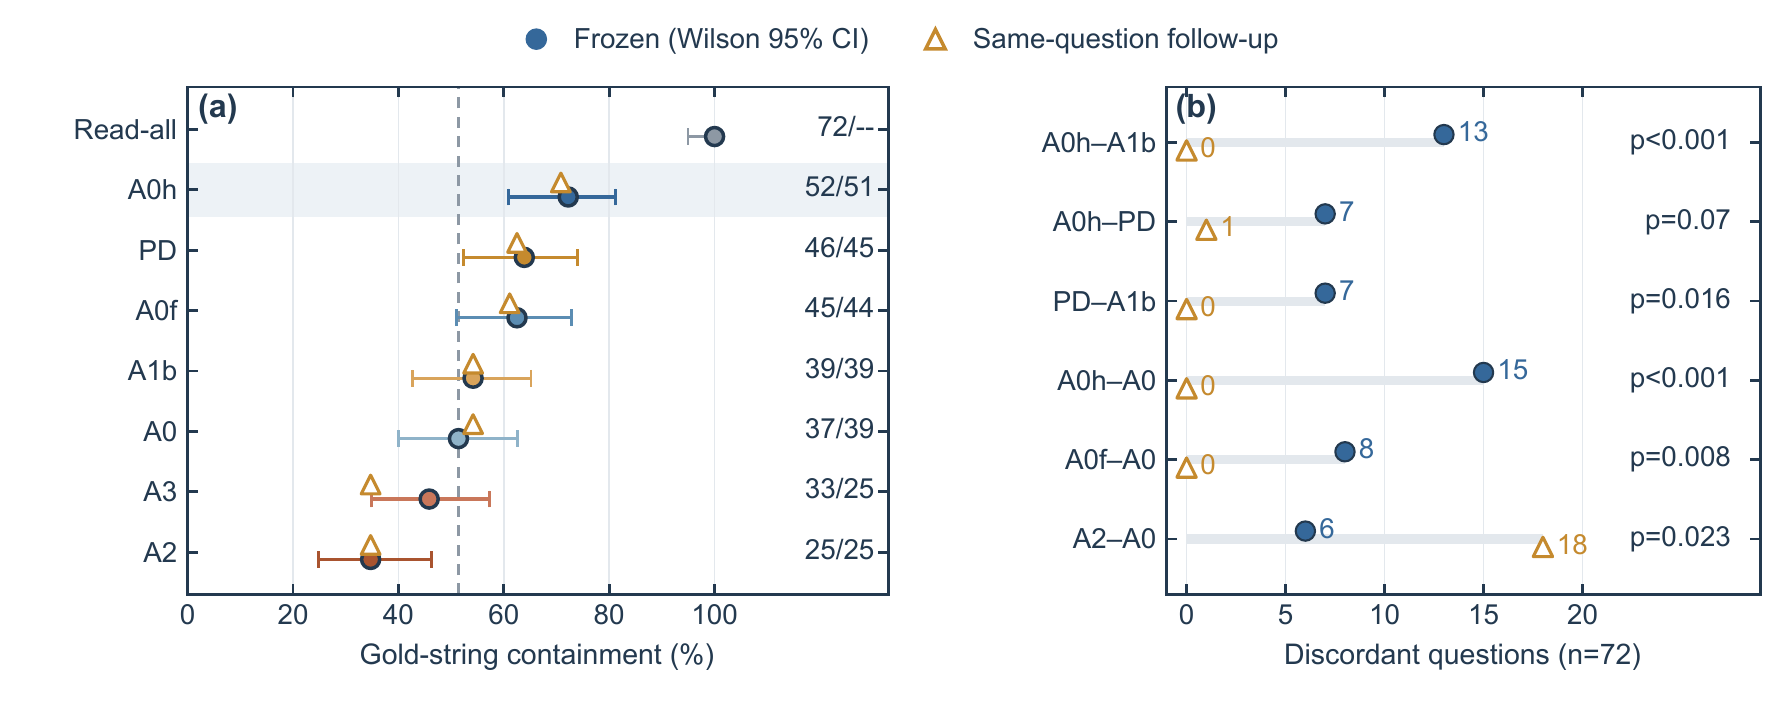
\includegraphics[width=6.45in]{figs/fig_opt_content.png}
\caption{\textbf{Figure 7.} Historical target-string containment on 72 in-domain questions;
the November~17 seven-arm rerun is not plotted.
(a) Frozen results with Wilson 95\% intervals (filled circles) and
same-question November~12 follow-up (open triangles). The dashed line marks
frozen A0. The frozen aggregate combines dates. The follow-up A3 ran
separately and read-all was incomplete. (b) Paired discordance in six frozen
contrasts. Circles and triangles count questions where only the first or
second arm contained the target, respectively. Exact McNemar $p$ values
are two-sided and unadjusted.}

\end{figure}


\subsection{8.7. E6: Answer and trace checks, abstention and cost}


Citation-marker counts differed across the three access paths in the original
grid and were equal in the repeat using the same five libraries. On ten research-paper
questions, the platform agent (P) produced nine answers with a
document-style marker, direct file tools (F) produced seven, and the
platform vector search over 800-character chunk copies (C) produced two.
In the repeat on the common libraries, each arm produced nine marker-bearing
answers (Figure~8). Across cells matched by question identifier,
nine answers gained a marker and none lost one. BQ06 was worded differently
between the two grids, however, and the access substrates also changed; the
counts therefore do not identify a causal effect of substrate or question
wording. The chunk arm's BQ04 answer, for
instance, named source paths without using a marker recognised by the
check. Tables~S7--S8 of the supplementary inventory audit source presence,
while Tables~S14--S15 report the individual and aggregate grid checks.

The gold identifier appeared in the answer or trace in all 60 cells of two
30-cell grids (ten questions, three arms per grid).
None of the 60 saved question texts contains its corresponding gold ID, so
the retained question fields do not support input-ID copying as an explanation
for this result. The ID check searches answer text and recorded tool-call
inputs and agent text; it does not establish source resolution or semantic
support. The original answers were rescored using revised BQ06 annotations;
under the original annotation the original P arm scored 10/10 strict, not
9/10. Under the revised 60\% keyword threshold, original-grid strict
coverage was 9/10 in each arm, and alias-aware coverage was 10/10 in each.
On the common substrate, strict coverage was 7/10 for P, 7/10 for F and
8/10 for C, and alias-aware coverage
was 9/10, 9/10 and 10/10. These string checks do not establish semantic
correctness. In the original grid, the platform agent took 52.6~s and cost
\$0.711 per question. The corresponding means were 22.2~s and \$0.487 for
F, and 24.5~s and \$0.527 for C. A separate later run on the repaired
platform had different keyword and more permissive marker rules and is not
comparable to the historical grids. Its mean wall-clock time was 131~s per
question and its total cost was \$3.10 for ten questions.

\textbf{Answer-level case study.} After ingesting DeepSeek-R1, two agent
harnesses answered four questions with the library, paper and source identifier
provided and the retrieval, judging and reading sequence prescribed.
The case review checked answer content, source provenance, quotations
and fabricated facts against the paper and passed all eight responses
(Table~S16). On the electricity-cost question, both responses identified
the reported \$294K GPU-rental training estimate and reported that the
paper supplied no electricity figure. Three further industrial-corpus
probes returned not-found. Related absent probes still yielded retrieval
candidates above the threshold (Fig.~S3).

\begin{figure}
\centering
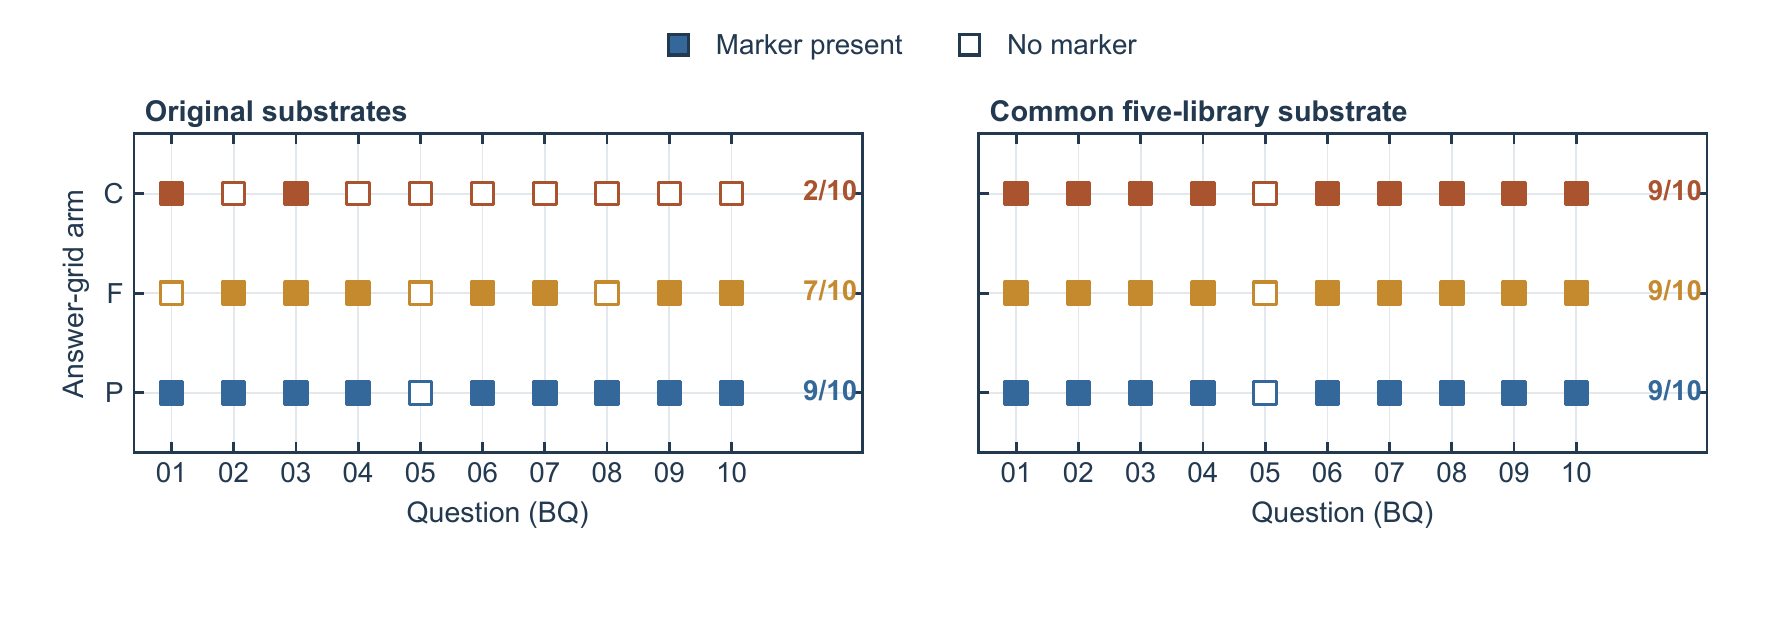
\includegraphics[width=6.45in]{figs/fig_opt_answer.png}
\caption{\textbf{Figure 8.} Document-style citation markers on two ten-question grids.
Each filled square represents one marker-bearing answer. (a) Original
grid with different access substrates. (b) Repeat on the same five
libraries. The gold identifier appeared in the answer or trace for
all 60 cells. The term-coverage counts are reported in Table~S15.
Each arm is a single execution.}

\end{figure}
\begin{figure}
\centering
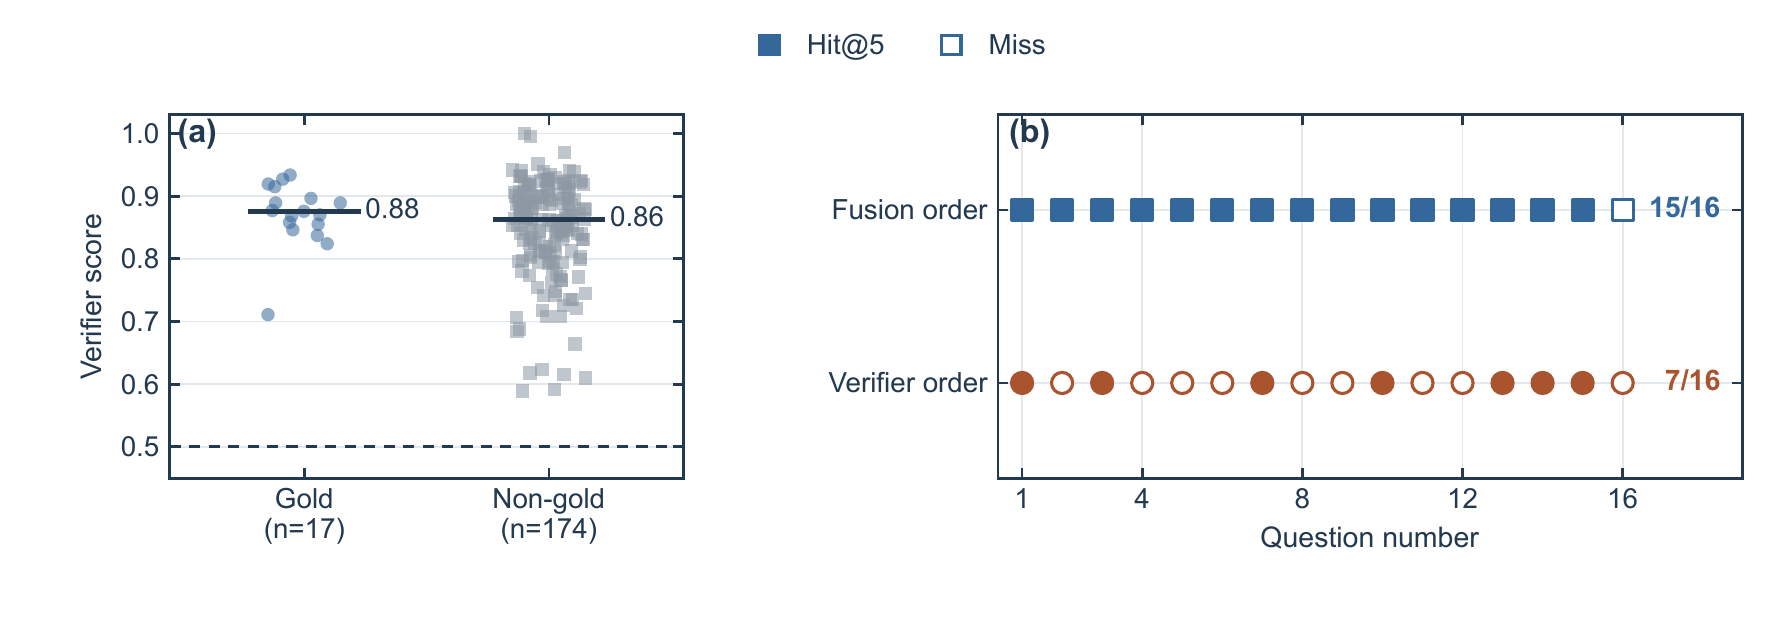
\includegraphics[width=6.45in]{figs/fig_opt_verifier.png}
\caption{\textbf{Figure 9.} Verifier scores and same-pool ordering from two separate
archives. (a) Laya scores for 191 recorded candidates across sixteen
hybrid runs. The 17 gold and 174 other scores have medians of 0.88 and
0.86, respectively. All recorded scores exceed 0.5, and one additional
Q14 candidate has no recorded score. Horizontal jitter separates the
marks. (b) Sixteen logged pools replayed in fusion and verifier order.
Filled marks indicate a gold document among the first five. Hit@5 is
15/16 in fusion order and 7/16 in verifier order.}

\end{figure}

\subsection{8.8. E7: Deployment-layer system arms and honesty contracts}

Three questions crossed pinned, unpinned and pinned hybrid-directed API
arms. The pinned arms returned both in-corpus gold identifiers, and all
three arms returned not-found for the out-of-corpus question. An unpinned
request exposed a transport limit. Its 131-document catalogue occupied
74.9~KB, exceeded the tool-output budget and yielded a truncated
preview, contributing to false refusals or stalled execution. Pagination and
grouped views let selected reruns complete, including the previously
failing query. A separate two-lane isolation test removed vector and
two-stage tools from one lane; its four initial traces recorded no vector-tool
calls, but none produced a final answer in that round. Catalogue truncation
was therefore not the only mechanism restricting access in these tests. In an
eighteen-arm battery, no final response contained a fabricated citation.
Interrupted arms were retried to produce one final response per condition.

\subsection{8.9. E8: When the verifier fails}


On sixteen logged pools from the historical hybrid wrapper, ordering
candidates by verifier score reduced Hit@5 from 15/16 in fusion order to
7/16 (Figure~9b). Holding the recorded pools fixed isolates
the effect of sorting these candidates. The Q2 record illustrates the
demotion (Fig.~S5). The gold root-cause report scored 0.846, below five
telemetry reports scoring 0.887--0.926, and fell from first in fusion order
to eighth.

In the separate score archive, all 191 recorded values exceeded the
0.5 admission threshold. One additional Q14 candidate had no recorded
score. The medians were 0.88 for 17 gold candidates and 0.86 for 174
others (Figure~9a). The candidate-level Mann--Whitney
test ($p=0.26$) ignores clustering by query. Replays using an NLI
checkpoint and span scoring yielded Hit@5 of 0.3125 and 0.1875. A
relative-margin replay preserved 16 of 17 golds at $m=0.15$ and all 17
at $m=0.20$, retaining 10.4 and 11.1 candidates on average, respectively.
Table~S6 of the supplementary inventory and Fig.~S4 give the threshold
and margin sweeps. The paper corpus did not exhibit the same top-five
loss, with domain, language and corpus size changing together. The
replay identifies a risk of using admission scores as a ranking
criterion in this pool. Because all logged scores exceeded the configured
threshold, the archive provides no observed effect of rejecting
candidates at that threshold.

\subsection{8.10. E9: Operational boundaries: stability, concurrency, gate and
scope ablations}

The 27-cell stability run recorded success across three tasks, three lanes
and three rounds; these execution statuses do not establish that all 27
answers were semantically correct. In a separate
single-instance read-ladder concurrency sweep, the loads were 90, 180 and
270 requests at 5, 15 and 30 clients. The read-ladder recorded zero errors,
with median latency rising from 5.2 to 1577~ms. A separate vector-only
probe at 30 clients and 9 requests/s completed 159 of 270 requests within
30~s; the other 111 were not completed in that window, and are not
classified here as explicit timeout responses. A cache repair lowered the
30-client median to 65.8~ms on selected read-ladder reruns. These are two
pressure-test protocols, not one combined error/timeout result; the full
sweep after repair, concurrent writes and crash recovery were outside that
retest.

An inspection of cross-library vector search identified eight collections
with unreadable index segments. The global response skipped those
collections and reported success without exposing incomplete coverage.
Scoped search found a document in a newly ingested affected library,
and forced reindexing restored its global hit. A scoped probe on a
different affected library also returned no results. The implementation
logs per-collection errors and continues with the other collections, so
a completed response can still represent partial coverage.

A reconstructed fixed-candidate gate replay used ten questions, up to twelve
candidates and an evidence cap of 4{,}000 characters. All three arms
packed the gold document first on the eight answerable questions.
Filtered and unfiltered document sets matched on nine questions, while
LLM grades differed on some of these questions (including $0\to5$ and
$3\to0$). Matching document sets does not establish that the evidence-pack
text was identical, so these grade changes cannot be attributed solely to
generation or grading variability. Both questions without a gold document
were refused in every
arm. In the separate routing probes, A0 yielded two empty survivor
lists in four cases, both without a top candidate. A0h yielded none.
These outcomes distinguish absent candidates from rejection at the gate.

In a separate scope check, pinning the gold library yielded Hit@5 of
8/8 on the paper-corpus questions with in-corpus gold documents. Pinning a
non-gold library yielded 0/8. Catalogue routing selected the correct
library first for six of the eight. Filenames bore domain prefixes,
and the unscoped path searched 20 live libraries, including 15 beyond
the evaluation corpus.


\section{9. Discussion and lessons learned}


The lifecycle audits show what a collection-level representation buys in
practice. A rename updated document state while leaving nine stale chunks
in the vector index. Re-indexing removed the duplicates and restored the
expected count. The three-source checks let operators verify the file,
registry and metadata views separately, while a search probe checks whether
the index reflects the change. The paper-ingestion audit reports separate
observations for a derived library and the five-library inventory
(Section~8.2). The practical implication is to
test retrieval after a lifecycle operation as well as checking its write
response. This joins metadata governance to a property that matters at
query time [3, 1].

At the access layer, the full route cards gave the scripted selector a
usable collection-level view. The evidence packs show a second decision
after routing: how much of the selected material to read. Adding document
and vector chunk windows in A0h raised target-string containment over A0 by
15 questions in the frozen run and 12 in each same-question rerun. The
frozen run used an average of 309~kB of trace-recorded text per question,
compared with 31.4~kB for A0 and 24.3~MB for the mechanical full read. Thus
A0h traded a larger reading budget for more retained targets while using
about 1.3\% of the full scan's text volume. A0h also led the per-library
union PD by six questions in both the frozen and November~12 records, with a smaller paired difference
that remained unresolved. PD searches each of the ten libraries separately
before merging document candidates. The stronger result is the improvement over A0
when the retrieval configuration expands the evidence it reads.

Source visibility carries through to answering. On different substrates,
the rates of detected document-style markers diverged across the three
interfaces. Counts were nine of ten for each arm in the repeat using the same
indexed libraries, but the changed BQ06 wording and access configurations
prevent attribution of that convergence to the substrate alone. Marker checks are a
trace-format diagnostic. A separate semantic assessment would be needed to
determine which answer claims the retrieved passages support.

The verifier replay identifies a distinct design choice. The same sixteen
candidate pools produced 15 top-five hits in fusion order and seven in
verifier-score order. Preserving candidate order after admission avoids
that specific failure mode. The score archive informs a separate question:
at the recorded threshold, all 191 scores passed, leaving the effect of
active filtering open. This separation is consistent with the practical
distinction between a relevance judgement and a ranking rule in work on
LLM judgements and reranking [58, 59].

Operational traces also show why a search needs to report its coverage.
Pagination recovered a failed catalogue path. An index read failure exposed
a different defect: the global channel could skip a library and still report
success. For the affected example, re-indexing recovered the missing hit.
Reporting partial coverage would help callers distinguish an incomplete search
from a completed search that returned no supporting evidence.


\section{10. Threats to validity}


\noindent\textbf{Data and scope.} The collections represent local
demonstration and benchmark workloads. Developers authored or expanded the
questions and gold annotations. The routing benchmark includes 52 expanded
questions, with 47 questions concentrated in three English domains.
Same-question reruns test repeatability under recorded changes to the
environment. An independent question set would test transfer. The storage
reconciliation examined 33 of 322 parts, and the four out-of-domain probes
characterise individual responses.

\noindent\textbf{Measurement and comparisons.} The content metric counts a
literal target string anywhere in the pack, including in a sibling
document. A post-hoc split by case-insensitive question--target overlap
(Section~8.1) gives frozen A0 and A0h containment of
16/29 and 21/29 on overlapping questions, and 21/43 and 31/43 on the
remainder. These are descriptive, non-random subsets, not a causal test of
overlap; lack of an exact match does not rule out other lexical cues.
Gold-ID checks search answers and recorded trace text; the saved grid
questions do not contain their corresponding IDs. Nevertheless, ID presence
does not establish source resolution or semantic correctness, and
claim-to-source support requires its own evaluation; citation markers only
indicate recognised formatting. The full-read comparator is a mechanical
scan of the corpus. Content arms change several components, including candidate
construction and reading scope. A0, A1b and A3 can use the gold domain when
resolving references, and A3 can fall back to descriptions or retrieve
outside the evaluated libraries. The archived traces leave the frequency of
these paths unknown. The reported contrasts therefore apply to the tested
configurations. A matched intervention would be needed to attribute
differences to navigation alone. The two ten-question answer grids use one
model and one run per arm, with the common-substrate grid controlling which
libraries each interface uses.

\noindent\textbf{Statistical and operational validity.} The paired
comparisons are exploratory. Wilson intervals summarise uncertainty
conditional on the question set and observed run. Candidate- and span-level
tests can understate uncertainty by treating within-query observations as
independent. Some historical reference-mode inputs, judge inputs and code
hashes are missing. The verifier results use a historical implementation
and support replay of the released records. The lifecycle assertions and
concurrency sweep cover one installation. The experience approval path,
multi-host reliability, and crash recovery remain open.


\section{11. Conclusion}


HMRS connects the state used to manage collections, documents and segments
to the interfaces that agents use to find and inspect evidence. The
collection catalogue and document shelf expose metadata for narrowing
search, and opened documents and indexed segments carry the provenance
needed to inspect a result. Lifecycle checks make discrepancies observable:
a rename left duplicate vector entries, and re-indexing restored the expected
state.

On the 72-question evaluation, the tiered configuration that combined
document and chunk windows returned packs containing more annotated target
strings than the baseline configuration. The difference was 15 questions in the
frozen run and 12 in each rerun on the same questions.
In the frozen trace, the combined configuration used a higher recorded text
volume than the baseline and less than the mechanical full scan; the scan was
incomplete or absent in the later runs. The verifier
replay exposed a complementary trade-off. Fusion order placed a gold
document in the top five for 15 of the 16 candidate pools, compared with
seven under verifier-score ordering.
These results motivate two concrete practices in managed document systems:
audit the state that supplies retrieval candidates, and test evidence
admission and ordering as separate decisions.



\section*{CRediT authorship contribution statement}
\textbf{Author 1:} Conceptualisation, Methodology, Software, Investigation,
Data curation, Writing -- original draft. \textbf{Author 2:} Validation,
Writing -- review \& editing, Supervision. 
\section*{Declaration of competing interest}
The authors declare that they have no known competing financial interests
or personal relationships that could have appeared to influence the work
reported in this paper.

\section*{Funding}
This research did not receive any specific grant from funding agencies in
the public, commercial, or not-for-profit sectors. 
\section*{Ethics statement}
This article does not report studies involving human participants, human
data, or animals.

\section*{Data availability}
The implementation and benchmark scripts are available at
\url{https://github.com/kingdol666/rag-knowledge}. The supplement describes
the campaigns and includes per-question results, provenance manifests and
the score and ordering records for the verifier replay. The accompanying
route and content trace CSVs report identifiers, containment outcomes, text
volumes and timings. These exports omit question text, reference strings and
returned passages; they support recomputation of reported summaries from saved
labels, not independent verification of every containment decision or a full
replay. Some historical verifier inputs and corpus/index states were not
retained. The source restrictions on the evaluation corpora limit
redistribution. The repository includes a recipe and synthetic sample for
constructing a substitute for the 42-document industrial demonstration
corpus.

\section*{Acknowledgments}
The authors thank the maintainers of the open-source components the platform
builds on. 
\section*{Declaration of generative AI and AI-assisted technologies in the manuscript preparation process}
Anthropic Claude Code, ZCode and OpenAI Codex assisted with language editing,
manuscript revision and preparation of tables from archived results. An AI
image tool assisted with initial figure concepts. The research uses of
language models are described with the retrieval workflow and experimental
design. The authors reviewed the manuscript and take responsibility for its
content.


\section*{References}

[1] T.~P{\"a}iv{\"a}rinta, B.~E. Munkvold, Enterprise content management: An integrated perspective on information management, in: Proc. 38th Annual Hawaii International Conference on System Sciences (HICSS), IEEE, 2005, pp. 96--96. \href {https://doi.org/10.1109/hicss.2005.244} {\texttt{doi:10.1109/hicss.2005.244}}.

[2] P.~Tyrv{\"a}inen, T.~P{\"a}iv{\"a}rinta, A.~Salminen, J.~Iivari, Characterizing the evolving research on enterprise content management, European Journal of Information Systems 15~(6) (2006) 627--634. \href {https://doi.org/10.1057/palgrave.ejis.3000648} {\texttt{doi:10.1057/palgrave.ejis.3000648}}.

[3] J.-R. Park, Metadata quality in digital repositories: A survey of the current state of the art, Cataloging \& Classification Quarterly 47~(3-4) (2009) 213--228. \href {https://doi.org/10.1080/01639370902737240} {\texttt{doi:10.1080/01639370902737240}}.

[4] S.~A. Golder, B.~A. Huberman, Usage patterns of collaborative tagging systems, Journal of Information Science 32~(2) (2006) 198--208. \href {https://doi.org/10.1177/0165551506062337} {\texttt{doi:10.1177/0165551506062337}}.

[5] J.~P. Callan, Z.~Lu, W.~B. Croft, Searching distributed collections with inference networks, in: Proc. of the 18th Annual International ACM SIGIR Conference (SIGIR '95), 1995, pp. 21--28. \href {https://doi.org/10.1145/215206.215328} {\texttt{doi:10.1145/215206.215328}}.

[6] L.~Si, J.~Callan, Relevant document distribution estimation method for resource selection, in: Proc. of the 26th Annual International ACM SIGIR Conference (SIGIR '03), 2003, pp. 298--305. \href {https://doi.org/10.1145/860435.860490} {\texttt{doi:10.1145/860435.860490}}.

[7] P.~Lewis, E.~Perez, A.~Piktus, F.~Petroni, V.~Karpukhin, N.~Goyal, H.~K{\"u}ttler, M.~Lewis, W.~Yih, T.~Rockt{\"a}schel, S.~Riedel, D.~Kiela, \href{https://proceedings.neurips.cc/paper/2020/hash/6b493230-Abstract.html}{Retrieval-augmented generation for knowledge-intensive {NLP} tasks}, in: Advances in Neural Information Processing Systems, Vol.~33, Curran Associates, Inc., 2020, pp. 9459--9474. URL \url{https://proceedings.neurips.cc/paper/2020/hash/6b493230-Abstract.html}

[8] V.~Karpukhin, B.~O{\u{g}}uz, S.~Min, P.~Lewis, L.~Wu, S.~Edunov, D.~Chen, W.~Yih, Dense passage retrieval for open-domain question answering, in: Proceedings of the 2020 Conference on Empirical Methods in Natural Language Processing ({EMNLP}), 2020, pp. 6769--6781. \href {https://doi.org/10.18653/v1/2020.emnlp-main.550} {\texttt{doi:10.18653/v1/2020.emnlp-main.550}}.

[9] Y.~Gao, Y.~Xiong, M.~Wang, H.~Wang, Modular {RAG}: Transforming {RAG} systems into {LEGO}-like reconfigurable frameworks, ACM Transactions on Information Systems 44 (2026) 1--53. \href {https://doi.org/10.1145/3837856} {\texttt{doi:10.1145/3837856}}.

[10] {Model Context Protocol Contributors}, Model context protocol specification (2025-11-25), \url{https://modelcontextprotocol.io/specification/2025-11-25}, accessed September 19, 2026; specification revision 2025-11-25 (2025).

[11] W.~Yang, L.~Some, M.~Bain, B.~Kang, A comprehensive survey on integrating large language models with knowledge-based methods, Knowledge-Based Systems 318 (2025) 113503. \href {https://doi.org/10.1016/j.knosys.2025.113503} {\texttt{doi:10.1016/j.knosys.2025.113503}}.

[12] S.~Auer, C.~Bizer, G.~Kobilarov, J.~Lehmann, R.~Cyganiak, Z.~Ives, {DBpedia}: A nucleus for a web of open data, in: The Semantic Web (ISWC/ASWC 2007), Lecture Notes in Computer Science, Springer, 2007, pp. 722--735. \href {https://doi.org/10.1007/978-3-540-76298-0_52} {\texttt{doi:10.1007/978-3-540-76298-0\_52}}.

[13] I.~Nonaka, A dynamic theory of organizational knowledge creation, Organization Science 5~(1) (1994) 14--37. \href {https://doi.org/10.1287/orsc.5.1.14} {\texttt{doi:10.1287/orsc.5.1.14}}.

[14] E.~Mosqueira-Rey, E.~Hern{\'a}ndez-Pereira, D.~Alonso-R{\'i}os, J.~Bobes-Bascar{\'a}n, {\'A}.~Fern{\'a}ndez-Leal, Human-in-the-loop machine learning: a state of the art, Artificial Intelligence Review 56~(4) (2022) 3005--3054. \href {https://doi.org/10.1007/s10462-022-10246-w} {\texttt{doi:10.1007/s10462-022-10246-w}}.

[15] F.~Sebastiani, Machine learning in automated text categorization, ACM Computing Surveys 34~(1) (2002) 1--47. \href {https://doi.org/10.1145/505282.505283} {\texttt{doi:10.1145/505282.505283}}.

[16] X.~Zhong, J.~Tang, A.~Jimeno~Yepes, {PubLayNet}: Largest dataset ever for document layout analysis, in: 2019 International Conference on Document Analysis and Recognition (ICDAR), IEEE, 2019, pp. 1015--1022. \href {https://doi.org/10.1109/icdar.2019.00166} {\texttt{doi:10.1109/icdar.2019.00166}}.

[17] Y.~Huang, T.~Lv, L.~Cui, Y.~Lu, F.~Wei, {LayoutLMv3}: Pre-training for document {AI} with unified text and image masking, in: Proc. 30th ACM International Conference on Multimedia (MM '22), ACM, 2022, pp. 4083--4091. \href {https://doi.org/10.1145/3503161.3548112} {\texttt{doi:10.1145/3503161.3548112}}.

[18] B.~Wang, C.~Xu, X.~Zhao, L.~Ouyang, F.~Wu, Z.~Zhao, R.~Xu, K.~Liu, Y.~Qu, F.~Shang, B.~Zhang, L.~Wei, Z.~Sui, W.~Li, B.~Shi, Y.~Qiao, D.~Lin, C.~He, {MinerU}: An open-source solution for precise document content extraction, arXiv preprint arXiv:2409.18839 (2024). \href {https://doi.org/10.48550/arXiv.2409.18839} {\texttt{doi:10.48550/arXiv.2409.18839}}.

[19] G.~S. Manku, A.~Jain, A.~Das~Sarma, Detecting near-duplicates for web crawling, in: Proc. 16th International Conference on World Wide Web (WWW '07), ACM, 2007, pp. 141--150. \href {https://doi.org/10.1145/1242572.1242592} {\texttt{doi:10.1145/1242572.1242592}}.

[20] P.~Missier, K.~Belhajjame, J.~Cheney, The {W3C} {PROV} family of specifications for modelling provenance metadata, in: Proc. 16th International Conference on Extending Database Technology (EDBT/ICDT '13), ACM, 2013, pp. 773--776. \href {https://doi.org/10.1145/2452376.2452478} {\texttt{doi:10.1145/2452376.2452478}}.

[21] J.~Cheney, L.~Chiticariu, W.-C. Tan, Provenance in databases: Why, how, and where, Foundations and Trends in Databases 1~(4) (2009) 379--474. \href {https://doi.org/10.1561/1900000006} {\texttt{doi:10.1561/1900000006}}.

[22] M.~Gallofr{\'e}~Oca{\~n}a, A.~L. Opdahl, {A Software Reference Architecture for Journalistic Knowledge Platforms}, Knowledge-Based Systems 276 (2023) 110750. \href {https://doi.org/10.1016/j.knosys.2023.110750} {\texttt{doi:10.1016/j.knosys.2023.110750}}.

[23] Y.~Yang, H.~Huang, Y.~Gao, J.~Li, {Building knowledge-grounded dialogue systems with graph-based semantic modelling}, Knowledge-Based Systems 298 (2024) 111943. \href {https://doi.org/10.1016/j.knosys.2024.111943} {\texttt{doi:10.1016/j.knosys.2024.111943}}.

[24] E.~Budur, R.~{\"O}z{\c{c}}elik, D.~Soylu, O.~Khattab, T.~G{\"u}ng{\"o}r, C.~Potts, {Building efficient and effective OpenQA systems for low-resource languages}, Knowledge-Based Systems 302 (2024) 112243. \href {https://doi.org/10.1016/j.knosys.2024.112243} {\texttt{doi:10.1016/j.knosys.2024.112243}}.

[25] I.~Aarab, {LLM-based IR-system for bank supervisors}, Knowledge-Based Systems 310 (2025) 112914. \href {https://doi.org/10.1016/j.knosys.2024.112914} {\texttt{doi:10.1016/j.knosys.2024.112914}}.

[26] G.~Ciatto, A.~Agiollo, M.~Magnini, A.~Omicini, {Large language models as oracles for instantiating ontologies with domain-specific knowledge}, Knowledge-Based Systems 310 (2025) 112940. \href {https://doi.org/10.1016/j.knosys.2024.112940} {\texttt{doi:10.1016/j.knosys.2024.112940}}.

[27] P.~Sarthi, S.~Abdullah, A.~Tuli, S.~Khanna, A.~Goldie, C.~D. Manning, \href{https://openreview.net/pdf?id=GN921JHCRw}{{RAPTOR}: Recursive abstractive processing for tree-organized retrieval}, in: The Twelfth International Conference on Learning Representations ({ICLR}), 2024. URL \url{https://openreview.net/pdf?id=GN921JHCRw}

[28] D.~Edge, H.~Trinh, N.~Cheng, J.~Bradley, A.~Chao, A.~Mody, S.~Truitt, D.~Metropolitansky, R.~O. Ness, J.~Larson, From local to global: A {Graph RAG} approach to query-focused summarization, arXiv preprint arXiv:2404.16130 (2024). \href {https://doi.org/10.48550/arXiv.2404.16130} {\texttt{doi:10.48550/arXiv.2404.16130}}.

[29] Z.~Guo, L.~Xia, Y.~Yu, T.~Ao, C.~Huang, {LightRAG}: Simple and fast retrieval-augmented generation, in: Findings of the Association for Computational Linguistics: EMNLP 2025, 2025, pp. 10746--10761. \href {https://doi.org/10.18653/v1/2025.findings-emnlp.568} {\texttt{doi:10.18653/v1/2025.findings-emnlp.568}}.

[30] Z.~Li, H.~Tian, L.~Luo, Y.~Cao, P.~Luo, {DeepRead}: Document structure-aware reasoning to enhance agentic search, arXiv preprint arXiv:2602.05014v3 (2026). \href {https://doi.org/10.48550/arXiv.2602.05014} {\texttt{doi:10.48550/arXiv.2602.05014}}.

[31] I.~H. Kinalioglu, {EPRAG}: An epistemic policy framework for action selection in multi-source enterprise retrieval-augmented generation, Knowledge-Based Systems 352 (2026) 116929. \href {https://doi.org/10.1016/j.knosys.2026.116929} {\texttt{doi:10.1016/j.knosys.2026.116929}}.

[32] S.~Robertson, H.~Zaragoza, The probabilistic relevance framework: {BM25} and beyond, Foundations and Trends in Information Retrieval 3~(4) (2009) 333--389. \href {https://doi.org/10.1561/1500000019} {\texttt{doi:10.1561/1500000019}}.

[33] M.-K. Ghali, A.~Farrag, D.~Won, Y.~Jin, Enhancing knowledge retrieval with in-context learning and semantic search through generative {AI}, Knowledge-Based Systems 311 (2025) 113047. \href {https://doi.org/10.1016/j.knosys.2025.113047} {\texttt{doi:10.1016/j.knosys.2025.113047}}.

[34] G.~V. Cormack, C.~L.~A. Clarke, S.~Buettcher, Reciprocal rank fusion outperforms {Condorcet} and individual rank learning methods, in: Proceedings of the 32nd International {ACM} {SIGIR} Conference on Research and Development in Information Retrieval, 2009, pp. 758--759. \href {https://doi.org/10.1145/1571941.1572114} {\texttt{doi:10.1145/1571941.1572114}}.

[35] J.~Chen, S.~Xiao, P.~Zhang, K.~Luo, D.~Lian, Z.~Liu, {M3-Embedding}: Multi-linguality, multi-functionality, multi-granularity text embeddings through self-knowledge distillation, in: Findings of the Association for Computational Linguistics: ACL 2024, Association for Computational Linguistics, 2024, pp. 2318--2335. \href {https://doi.org/10.18653/v1/2024.findings-acl.137} {\texttt{doi:10.18653/v1/2024.findings-acl.137}}.

[36] F.~Li, X.~Li, J.~Bao, Recursive multi-modal retrieval for structured semantic trees in engineering documents, Knowledge-Based Systems 338 (2026) 115433. \href {https://doi.org/10.1016/j.knosys.2026.115433} {\texttt{doi:10.1016/j.knosys.2026.115433}}.

[37] T.~Chen, H.~Wang, S.~Chen, W.~Yu, K.~Ma, X.~Zhao, H.~Zhang, D.~Yu, Dense x retrieval: What retrieval granularity should we use?, in: Proc. of EMNLP 2024, 2024, pp. 15159--15177. \href {https://doi.org/10.18653/v1/2024.emnlp-main.845} {\texttt{doi:10.18653/v1/2024.emnlp-main.845}}.

[38] J.~Shen, H.~Zhu, B.~Zhang, Toward trustworthy engineering information extraction using retrieval-augmented generation, Knowledge-Based Systems 348 (2026) 116418. \href {https://doi.org/10.1016/j.knosys.2026.116418} {\texttt{doi:10.1016/j.knosys.2026.116418}}.

[39] Y.~Xu, H.~Liang, J.~Li, S.~Xu, Q.~Chen, Q.~Zhang, C.~Li, Z.~Yang, F.~Yang, Y.~Yang, P.~Cheng, M.~Yang, Spfresh: Incremental in-place update for billion-scale vector search, in: Proc. of the 29th Symposium on Operating Systems Principles (SOSP '23), 2023, pp. 545--561. \href {https://doi.org/10.1145/3600006.3613166} {\texttt{doi:10.1145/3600006.3613166}}.

[40] S.~Yao, J.~Zhao, D.~Yu, N.~Du, I.~Shafran, K.~Narasimhan, Y.~Cao, \href{https://openreview.net/pdf?id=WE_vluYUL-X}{{ReAct}: Synergizing reasoning and acting in language models}, in: The Eleventh International Conference on Learning Representations ({ICLR}), 2023. URL \url{https://openreview.net/pdf?id=WE_vluYUL-X}

[41] T.~Schick, J.~Dwivedi-Yu, R.~Dess{\`i}, R.~Raileanu, M.~Lomeli, E.~Hambro, L.~Zettlemoyer, N.~Cancedda, T.~Scialom, Toolformer: Language models can teach themselves to use tools, in: Advances in Neural Information Processing Systems, Vol.~36, 2023, pp. 68539--68551. \href {https://doi.org/10.52202/075280-2997} {\texttt{doi:10.52202/075280-2997}}.

[42] L.~Siddharth, J.~Luo, {Retrieval augmented generation using engineering design knowledge}, Knowledge-Based Systems 303 (2024) 112410. \href {https://doi.org/10.1016/j.knosys.2024.112410} {\texttt{doi:10.1016/j.knosys.2024.112410}}.

[43] Z.~Peng, X.~Wu, Q.~Wang, Y.~Fang, {Soft prompt tuning for augmenting dense retrieval with large language models}, Knowledge-Based Systems 309 (2025) 112758. \href {https://doi.org/10.1016/j.knosys.2024.112758} {\texttt{doi:10.1016/j.knosys.2024.112758}}.

[44] L.~Massai, {Evaluation of semantic relations impact in query expansion-based retrieval systems}, Knowledge-Based Systems 283 (2024) 111183. \href {https://doi.org/10.1016/j.knosys.2023.111183} {\texttt{doi:10.1016/j.knosys.2023.111183}}.

[45] D.~Tao, C.~Wang, F.~Huang, J.~Chen, Y.~Huang, M.~Jiang, {Fine-grained Stateful Knowledge Exploration: Effective and efficient graph retrieval with Large Language Models}, Knowledge-Based Systems 326 (2025) 114011. \href {https://doi.org/10.1016/j.knosys.2025.114011} {\texttt{doi:10.1016/j.knosys.2025.114011}}.

[46] C.~Packer, S.~Wooders, K.~Lin, V.~Fang, S.~G. Patil, I.~Stoica, J.~E. Gonzalez, {MemGPT}: Towards {LLMs} as operating systems, arXiv preprint arXiv:2310.08560 (2023). \href {https://doi.org/10.48550/arXiv.2310.08560} {\texttt{doi:10.48550/arXiv.2310.08560}}.

[47] W.~Xu, Z.~Liang, K.~Mei, H.~Gao, J.~Tan, Y.~Zhang, {A-MEM}: Agentic memory for {LLM} agents, in: Advances in Neural Information Processing Systems, Vol.~38, 2025, pp. 20004--20031. \href {https://doi.org/10.52202/085713-0593} {\texttt{doi:10.52202/085713-0593}}.

[48] A.~Miles, S.~Bechhofer, {SKOS} simple knowledge organization system reference, W3C Recommendation, \url{https://www.w3.org/TR/skos-reference/} (2009).

[49] {DCMI Usage Board}, \href{https://www.dublincore.org/specifications/dublin-core/dcmi-terms/2020-01-20/}{{DCMI} metadata terms}, DCMI Recommendation (2020). URL \url{https://www.dublincore.org/specifications/dublin-core/dcmi-terms/2020-01-20/}

[50] A.~Asai, Z.~Wu, Y.~Wang, A.~Sil, H.~Hajishirzi, \href{https://openreview.net/pdf?id=hSyW5go0v8}{{Self-RAG}: Learning to retrieve, generate, and critique through self-reflection}, in: The Twelfth International Conference on Learning Representations ({ICLR}), 2024. URL \url{https://openreview.net/pdf?id=hSyW5go0v8}

[51] S.-Q. Yan, J.-C. Gu, Y.~Zhu, Z.-H. Ling, Corrective retrieval augmented generation, in: Findings of the Association for Computational Linguistics: IJCNLP-AACL 2026, 2026, pp. 2991--3003. \href {https://doi.org/10.18653/2026.findings-aacl.151} {\texttt{doi:10.18653/2026.findings-aacl.151}}.

[52] Z.~Jiang, F.~Xu, L.~Gao, Z.~Sun, Q.~Liu, J.~Dwivedi-Yu, Y.~Yang, J.~Callan, G.~Neubig, Active retrieval augmented generation, in: Proceedings of the 2023 Conference on Empirical Methods in Natural Language Processing ({EMNLP}), 2023, pp. 7969--7992. \href {https://doi.org/10.18653/v1/2023.emnlp-main.495} {\texttt{doi:10.18653/v1/2023.emnlp-main.495}}.

[53] A.~Kamath, R.~Jia, P.~Liang, Selective question answering under domain shift, in: Proceedings of the 58th Annual Meeting of the Association for Computational Linguistics ({ACL}), 2020, pp. 5684--5696. \href {https://doi.org/10.18653/v1/2020.acl-main.503} {\texttt{doi:10.18653/v1/2020.acl-main.503}}.

[54] S.~Feng, W.~Shi, Y.~Wang, W.~Ding, V.~Balachandran, Y.~Tsvetkov, Don't hallucinate, abstain: Identifying {LLM} knowledge gaps via multi-{LLM} collaboration, in: Proceedings of the 62nd Annual Meeting of the Association for Computational Linguistics (ACL), 2024, pp. 14664--14690. \href {https://doi.org/10.18653/v1/2024.acl-long.786} {\texttt{doi:10.18653/v1/2024.acl-long.786}}.

[55] Z.~Yin, Q.~Sun, Q.~Guo, J.~Wu, X.~Qiu, X.~Huang, Do large language models know what they don't know?, in: Findings of the Association for Computational Linguistics: ACL 2023, 2023, pp. 8653--8665. \href {https://doi.org/10.18653/v1/2023.findings-acl.551} {\texttt{doi:10.18653/v1/2023.findings-acl.551}}.

[56] N.~F. Liu, T.~Zhang, P.~Liang, Evaluating verifiability in generative search engines, in: Findings of the Association for Computational Linguistics: EMNLP 2023, 2023, pp. 7001--7025. \href {https://doi.org/10.18653/v1/2023.findings-emnlp.467} {\texttt{doi:10.18653/v1/2023.findings-emnlp.467}}.

[57] T.~Gao, H.~Yen, J.~Yu, D.~Chen, Enabling large language models to generate text with citations, in: Proceedings of the 2023 Conference on Empirical Methods in Natural Language Processing (EMNLP), 2023, pp. 6465--6488. \href {https://doi.org/10.18653/v1/2023.emnlp-main.398} {\texttt{doi:10.18653/v1/2023.emnlp-main.398}}.

[58] L.~Zheng, W.-L. Chiang, Y.~Sheng, S.~Zhuang, Z.~Wu, Y.~Zhuang, Z.~Lin, Z.~Li, D.~Li, E.~Xing, H.~Zhang, J.~E. Gonzalez, I.~Stoica, Judging {LLM}-as-a-judge with {MT-Bench} and {Chatbot Arena}, in: Advances in Neural Information Processing Systems (NeurIPS), Vol.~36, 2023, pp. 46595--46623. \href {https://doi.org/10.52202/075280-2020} {\texttt{doi:10.52202/075280-2020}}.

[59] W.~Sun, L.~Yan, X.~Ma, S.~Wang, P.~Ren, Z.~Chen, D.~Yin, Z.~Ren, Is {ChatGPT} good at search? investigating large language models as {Re-Ranking Agents}, in: Proceedings of the 2023 Conference on Empirical Methods in Natural Language Processing (EMNLP), 2023, pp. 14918--14937. \href {https://doi.org/10.18653/v1/2023.emnlp-main.923} {\texttt{doi:10.18653/v1/2023.emnlp-main.923}}.

[60] A.~Panickssery, S.~R. Bowman, S.~Feng, {LLM} evaluators recognize and favor their own generations, in: Advances in Neural Information Processing Systems (NeurIPS), Vol.~37, 2024, pp. 68772--68802. \href {https://doi.org/10.52202/079017-2197} {\texttt{doi:10.52202/079017-2197}}.

[61] Z.~Zhou, M.~Li, X.~Fang, X.~Zhou, W.~Lin, Z.~Zheng, {LGMT: Logic-Grounded Metamorphic Testing for evaluating the reasoning reliability of LLMs}, Knowledge-Based Systems 348 (2026) 116324. \href {https://doi.org/10.1016/j.knosys.2026.116324} {\texttt{doi:10.1016/j.knosys.2026.116324}}.

[62] {Convai Innovations}, \href{https://huggingface.co/convaiinnovations/laya}{Laya model card}, accessed November 18, 2026. URL \url{https://huggingface.co/convaiinnovations/laya}

[63] {Chroma}, \href{https://docs.trychroma.com/docs/overview/introduction}{Chroma documentation: Introduction}, accessed November 18, 2026. URL \url{https://docs.trychroma.com/docs/overview/introduction}

[64] Y.~A. Malkov, D.~A. Yashunin, Efficient and robust approximate nearest neighbor search using hierarchical navigable small world graphs, IEEE Transactions on Pattern Analysis and Machine Intelligence 42~(4) (2020) 824--836. \href {https://doi.org/10.1109/TPAMI.2018.2889473} {\texttt{doi:10.1109/TPAMI.2018.2889473}}.

[65] {Neo4j, Inc.}, \href{https://neo4j.com/docs/operations-manual/current/}{{Neo4j} operations manual}, accessed November 18, 2026. URL \url{https://neo4j.com/docs/operations-manual/current/}

[66] N.~Craswell, B.~Mitra, E.~Yilmaz, D.~Campos, J.~Lin, {MS MARCO}: Benchmarking ranking models in the large-data regime, in: Proc. 44th International ACM SIGIR Conference (SIGIR '21), ACM, 2021, pp. 1566--1576. \href {https://doi.org/10.1145/3404835.3462804} {\texttt{doi:10.1145/3404835.3462804}}.

[67] S.~Es, J.~James, L.~Espinosa~Anke, S.~Schockaert, {RAGAs}: Automated evaluation of retrieval augmented generation, in: Proc. 18th Conference of the European Chapter of the ACL: System Demonstrations, ACL, 2024, pp. 150--158. \href {https://doi.org/10.18653/v1/2024.eacl-demo.16} {\texttt{doi:10.18653/v1/2024.eacl-demo.16}}.

[68] J.~Saad-Falcon, O.~Khattab, C.~Potts, M.~Zaharia, {ARES}: An automated evaluation framework for retrieval-augmented generation systems, in: Proc. 2024 Conference of the North American Chapter of the ACL: Human Language Technologies (Vol. 1: Long Papers), ACL, 2024, pp. 338--354. \href {https://doi.org/10.18653/v1/2024.naacl-long.20} {\texttt{doi:10.18653/v1/2024.naacl-long.20}}.

[69] K.~J{\"a}rvelin, J.~Kek{\"a}l{\"a}inen, Cumulated gain-based evaluation of {IR} techniques, ACM Transactions on Information Systems 20~(4) (2002) 422--446. \href {https://doi.org/10.1145/582415.582418} {\texttt{doi:10.1145/582415.582418}}.
\end{document}
